%%%%%%%%%%%%%%%%%%%%%%%%%%%%%%%%%%%%%%%%%%%%%%%%%%%%%%%%%%%%%%%%%%%%%%%%%%%%%%%%%%%%%%%
%\chapter[Système du 1er et 2nd ordre]{Système linéaire du premier et du second ordre\label{chap-1er2nd}}
\chapter[Modélisation des SLCI]{Modélisation des SLCI\label{chap-model} et leurs réponses temporelles}
%%%%%%%%%%%%%%%%%%%%%%%%%%%%%%%%%%%%%%%%%%%%%%%%%%%%%%%%%%%%%%%%%%%%%%%%%%%%%%%%%%%%%%%
\minitoc
\newpage
%%%%%%%%%%%%%%%%%%%%%%%%%%%%%%%%%%%%%%%%%%%%%%%%%%%%%%%%%%%%%%%%%%%%%%%%%%%%%%%%%%%%%%%
\section{Introduction}
%%%%%%%%%%%%%%%%%%%%%%%%%%%%%%%%%%%%%%%%%%%%%%%%%%%%%%%%%%%%%%%%%%%%%%%%%%%%%%%%%%%%%%%

Dans ce chapitre, nous allons étudier la réponse 
temporelle de différents systèmes modèles. Ces modèles sont 
\begin{itemize}
    \item les systèmes du \textbf{premier ordre},
    \item les systèmes du \textbf{second ordre},
    \item les systèmes gain, intégrateur, dérivateur et retard purs.
\end{itemize}
Ces modèles reflètent les différentes équations différentielles et 
systèmes physiques généralement rencontrés dans la nature.
Les deux plus importants sont les systèmes du premier et second ordre 
qui sont pour cette raison éxaminer en détail. 
Nous généraliserons aux systèmes d'ordre supérieur en montrant 
que toute fonction de transferts peut se factoriser en un produit
de ces systèmes modèles.

Nous suivrons la même présentation pour tous les modèles: 
nous donnerons d'abord l'équation différentielle régissant le système, puis 
sa fonction de transfert ainsi que ses pôles, avant de 
déterminer analytiquement les différentes réponses temporelles : i
impulsionnelle, indicielle et la réponse à une rampe. 
Le principal objectif de cette étude est d'établir les caractéristiques 
de ces modèles à partir de leurs réponses temporelles.

\newpage
%%%%%%%%%%%%%%%%%%%%%%%%%%%%%%%%%%%%%%%%%%%%%%%%%%%%%%%%%%%%%%%%%%%%%%%%%%%%%%%%%%%%%%%
\section{Système du premier ordre}
%%%%%%%%%%%%%%%%%%%%%%%%%%%%%%%%%%%%%%%%%%%%%%%%%%%%%%%%%%%%%%%%%%%%%%%%%%%%%%%%%%%%%%%

%%%%%%%%%%%%%%%%%%%%%%%%%%%%%%%%%%%%%%%%%%%%%%%%%%%%%%%%%%%%%%%%%%%%%%%%%%%%%%%%%%%%%%%
\subsection{Définition d'un système du premier ordre}
%%%%%%%%%%%%%%%%%%%%%%%%%%%%%%%%%%%%%%%%%%%%%%%%%%%%%%%%%%%%%%%%%%%%%%%%%%%%%%%%%%%%%%%
\index{Système du premier ordre!définition}
Un système du premier ordre est un système régit par une équation
différentielle linéaire à coefficient constant du premier ordre 
(i.e $n=1$ pour l'\cref{eq-difflci}), de la forme générale :
\begin{bequation}[ams align]
    \tau\devi{s(t)}{}+s(t)=K e(t)\label{eq-1er}
\end{bequation}
où $K$ est le gain statique et $\tau>0$ la constante de 
temps du système. La condition sur le signe de $\tau$ sera 
discutée au moment de l'établissement des réponses temporelles.
L'analyse dimentionnelle de cette équation différentielle, nous permet 
de confirmer que $\tau$ à la dimension d'un temps, mais surtout que 
la dimension du gain statique est donnée par le rapport des dimensions de 
la sortie sur l'entrée. Autrement dit, c'est un paramètre sans dimension 
c'est l'entrée et la sortie sont de même nature.


%%%%%%%%%%%%%%%%%%%%%%%%%%%%%%%%%%%%%%%%%%%%%%%%%%%%%%%%%%%%%%%%%%%%%%%%%%%%%%%%%%%%%%%
\subsection{Fonction de transfert d'un système du premier ordre}
%%%%%%%%%%%%%%%%%%%%%%%%%%%%%%%%%%%%%%%%%%%%%%%%%%%%%%%%%%%%%%%%%%%%%%%%%%%%%%%%%%%%%%%
\index{Système du premier ordre!fonction de transfert}
La transformée de Laplace de l'\cref{eq-1er}, dans les conditions de Heaviside, nous donne :
$$
\tau pS(p)+S(p)=KE(p)
$$
La fonction de transfert $H(p)$ d'un système du premier ordre est donc de la forme:
\begin{bequation}[ams align]
    H(p)=\dfrac{S(p)}{E(p)}=\dfrac{K}{\tau p + 1}\label{eq-ft1er}
\end{bequation}

%%%%%%%%%%%%%%%%%%%%%%%%%%%%%%%%%%%%%%%%%%%%%%%%%%%%%%%%%%%%%%%%%%%%%%%%%%%%%%%%%%%%%%%
\subsection{Pôle de la fonction de transfert du premier ordre}
%%%%%%%%%%%%%%%%%%%%%%%%%%%%%%%%%%%%%%%%%%%%%%%%%%%%%%%%%%%%%%%%%%%%%%%%%%%%%%%%%%%%%%%
Un système du premier ordre ne possède qu'un seul pôle qui est trivialement 
déterminé par la résolution de l'équation :
$$
\tau p + 1 =0
$$
ce pôle $p_1=-\dfrac{1}{\tau}$ est donc réel négatif pour $\tau>0$.
La fonction de transfert d'un système du premier peut alors s'écrire 
sous la forme factorisée suivante
$$
H(p)=\dfrac{K}{(p-p_1)}=\dfrac{K}{\tau\left(p+\dfrac{1}{\tau}\right)}.
$$

%%%%%%%%%%%%%%%%%%%%%%%%%%%%%%%%%%%%%%%%%%%%%%%%%%%%%%%%%%%%%%%%%%%%%%%%%%%%%%%%%%%%%%%
\subsection{Réponses temporelles d'un système du premier ordre}
%%%%%%%%%%%%%%%%%%%%%%%%%%%%%%%%%%%%%%%%%%%%%%%%%%%%%%%%%%%%%%%%%%%%%%%%%%%%%%%%%%%%%%%
Nous allons maintenant établir les réponses temporelles d'un système 
du premier ordre aux signaux usuels présentés au chapitre~\cref{chap_slci}.

\begin{figure}[!t]
\begin{center}
    \tikzsetnextfilename{1er_imp-chap2_ext}
    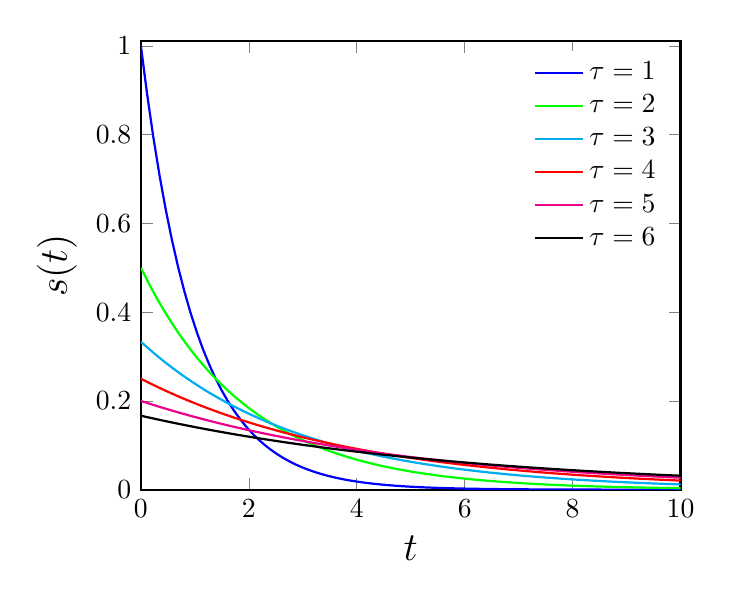
\begin{tikzpicture}
        \begin{axis}[
        legend style={draw=none},
        axis line style = thick,
        %height=7cm,
        %width=9cm,
        xmin=0,
        xmax=10,
        ymin=0,
        ymax=1.01,
        xlabel={$t$},
        ylabel={$s(t)$},
        label style={font=\Large},
        ]
            \addplot [thick,color=blue,domain=0:11.5, samples=101,unbounded coords=jump]{exp(-x)};
            \addplot [thick,color=green,domain=0:11.5, samples=101,unbounded coords=jump]{(exp(-x/2))/2};
            \addplot [thick,color=cyan,domain=0:11.5, samples=101,unbounded coords=jump]{(exp(-x/3))/3};
            \addplot [thick,color=red,domain=0:11.5, samples=101,unbounded coords=jump]{(exp(-x/4))/4};
            \addplot [thick,color=magenta,domain=0:11.5, samples=101,unbounded coords=jump]{(exp(-x/5))/5};
            \addplot [thick,color=black,domain=0:11.5, samples=101,unbounded coords=jump]{(exp(-x/6))/6};
        \legend{$\tau=1$,$\tau=2$,$\tau=3$,$\tau=4$,$\tau=5$,$\tau=6$}
        \end{axis}
    \end{tikzpicture}
\caption{Réponse impulsionnelle d'un système du premier ordre pour différentes valeurs
    de la constante de temps $\tau$  (\Cref{eq-1er_imp}) avec $K=1$ et $E_0=1$.\label{fig-1er_imp}}
\end{center}
\end{figure}

%%%%%%%%%%%%%%%%%%%%%%%%%%%%%%%%%%%%%%%%%%%%%%%%%%%%%%%%%%%%%%%%%%%%%%%%%%%%%%%%%%%%%%%
\subsubsection{Réponse impulsionnelle}
%%%%%%%%%%%%%%%%%%%%%%%%%%%%%%%%%%%%%%%%%%%%%%%%%%%%%%%%%%%%%%%%%%%%%%%%%%%%%%%%%%%%%%%
\index{Système du premier ordre!réponse impulsionnelle}
Nous condidérons une excitation impulsionnelle de la forme :
$$
e(t)=E_0\delta(t),
$$
où $\delta(t)$ est l'impulsion de Dirac et $E_0$ est une constante.

La réponse impulsionnelle d'un système du premier ordre est, dans le domaine de Laplace,
de la forme :
$$
S(p)=H(p)E(p)=\dfrac{KE_0}{(\tau p+1)}.
$$
La transformée de Laplace inverse de $S(p)$ (c.f ligne 7 du tableau de l'\cref{annexe-lap}),
nous donne la forme générale de la réponse impulsionnelle d'un système du premier ordre:
\begin{bequation}[ams align]
    \laplacei{S(p)}=s(t)=\dfrac{KE_0}{\tau} e^{-t/\tau}\label{eq-1er_imp}.
\end{bequation}
Cette réponse correspond à une simple exponentielle décroissante pour $\tau>0$.
La~\cref{fig-1er_imp} présente la réponse impulsionnelle d'un système du premier ordre pour
différentes valeurs de la constante de temps $\tau$.
On observe que pour $t\to\infty$, la valeur de $s(t)$ tend vers 0, ce qui est caractéristique 
d'un système stable. Nous pouvons donc considérer que $\tau$ est strictement positif pour 
une question de stabilité.  

Il est également possible d'observer que la pente à l'origine dépend de la constante de temps.
La pente à l'origine peut être obtenue directement en dérivant la réponse temporelle $s(t)$
$$
s'(0)=-\dfrac{KE_0}{\tau^2}
$$
La pente à l'origine est négative et inversemment proportionnelle 
au carré de la constante de temps du système $\tau$.

Le~\cref{tab-1er_imp} donne quelques valeurs particulières de la réponse impulsionnelle. 
D'après celui-ci, on constate que le temps $t_{5\%}$ de réponse à 5\% est de l'ordre 
de 3$\tau$ (i.e $-\log{5\%}$). Le transitoire est lui de l'ordre de $7\tau$ 
(c'est à dire le temps à partir duquel on considère que le signal est nul).

\begin{table}
    \begin{center}
		\begin{tabular}{M{2cm}M{2cm}M{2.0cm}M{2.0cm}M{2cm}N}
        \hhline{=====}
								 & $t=0.5\tau$    & $t=\tau$    & $t=3\tau$ & $t=7\tau$ & \\[1.5em]
        \hline
		$\dfrac{s(t)}{KE_0}$     & 0.606          & 0.368       & 0.05      & $\sim$ 0& \\ [1.5em]
        \hhline{=====}
    \end{tabular}
    \caption{Quelques valeurs particulières de la réponse impulsionnelle d'un système du premier ordre\label{tab-1er_imp}.}
    \end{center}
\end{table}


%%%%%%%%%%%%%%%%%%%%%%%%%%%%%%%%%%%%%%%%%%%%%%%%%%%%%%%%%%%%%%%%%%%%%%%%%%%%%%%%%%%%%%%
\begin{figure}
\centering
\tikzsetnextfilename{1er_ind1-chap2_ext}
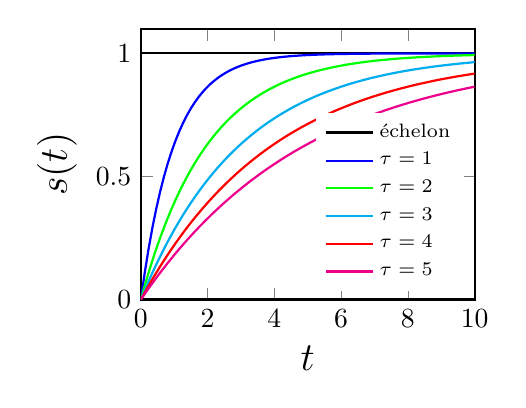
\begin{tikzpicture}
\begin{axis}[%
    legend style={draw=none,font=\scriptsize},
    legend pos=south east,
    axis line style = thick,
    width=0.48\textwidth,
    xmin=0,
    xmax=10,
    ymin=0,
    ymax=1.1,
    xlabel={$t$},
    ylabel={$s(t)$},
    label style={font=\Large},
    legend cell align={left},
]%
\addplot[thick,color=black,domain=0:11.5, samples=101,unbounded coords=jump] {{1}};
\addplot[thick,color=blue,domain=0:11.5, samples=101,unbounded coords=jump]{1-exp(-x)};
\addplot[thick,color=green,domain=0:11.5, samples=101,unbounded coords=jump]{(1-exp(-x/2))};
\addplot[thick,color=cyan,domain=0:11.5, samples=101,unbounded coords=jump]{(1-exp(-x/3))};
\addplot[thick,color=red,domain=0:11.5, samples=101,unbounded coords=jump]{(1-exp(-x/4))};
\addplot[thick,color=magenta,domain=0:11.5, samples=101,unbounded coords=jump]{(1-exp(-x/5))};
\legend{échelon,$\tau=1$,$\tau=2$,$\tau=3$,$\tau=4$,$\tau=5$}
\end{axis}%
\end{tikzpicture}%
\hfill
\tikzsetnextfilename{1er_ind2-chap2_ext}
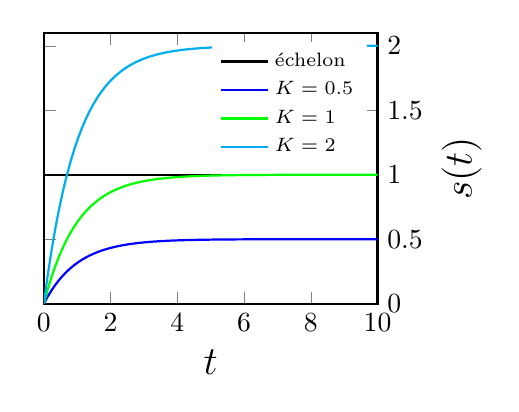
\begin{tikzpicture}
\begin{axis}[
    legend style={draw=none,font=\scriptsize},
    legend pos=north east,
    axis line style = thick,
    width=0.48\textwidth,
    xmin=0,
    xmax=10,
    ymin=0,
    ymax=2.1,
    xlabel={$t$},
    ylabel={$s(t)$},
    ylabel near ticks, yticklabel pos=right,
    label style={font=\Large},
    legend cell align={left},
]%
\addplot[thick,color=black,domain=0:11.5, samples=101,unbounded coords=jump]{{1}};%
\addplot[thick,color=blue,domain=0:11.5, samples=101,unbounded coords=jump]{0.5*(1-exp(-x))};
\addplot[thick,color=green,domain=0:11.5, samples=101,unbounded coords=jump]{1-exp(-x)};
\addplot[thick,color=cyan,domain=0:11.5, samples=101,unbounded coords=jump]{2*(1-exp(-x))};
\legend{échelon,$K=0.5$,$K=1$,$K=2$}
\end{axis}
\end{tikzpicture}
\caption{Réponse indicielle d'un système du premier ordre avec $E_0=1$. (gauche) 
         Pour différentes valeurs de $\tau$ et avec $K=1$. (droite) Pour différentes 
         valeurs du gain $K$ et avec $\tau=1$.\label{fig-1er_ind}}
\end{figure}
%%%%%%%%%%%%%%%%%%%%%%%%%%%%%%%%%%%%%%%%%%%%%%%%%%%%%%%%%%%%%%%%%%%%%%%%%%%%%%%%%%%%%%%
\subsubsection{Réponse indicielle}
%%%%%%%%%%%%%%%%%%%%%%%%%%%%%%%%%%%%%%%%%%%%%%%%%%%%%%%%%%%%%%%%%%%%%%%%%%%%%%%%%%%%%%%
\index{Système du premier ordre!réponse indicielle}

Pour déterminer la réponse indicielle, nous considérons une entrée $e(t)$ en échelon telle que :
$$
e(t)=E_0\cdot u(t),
$$
où $u(t)$ est l'échelon unitaire et $E_0$ est une constante.

Dans le domaine de Laplace la sortie est donc de la forme :
$$
S(p)=H(p)E(p)=\dfrac{KE_0}{p(1+\tau p)}=\dfrac{KE_0}{\tau p(p+\frac{1}{\tau})}
$$
La transformée de Laplace inverse de $S(p)$ (c.f ligne 11 du tableau de l'\cref{annexe-lap}),
nous donne la forme générale de la réponse indicielle d'un système du premier ordre:
\begin{bequation}[ams align]
\laplacei{S(p)}=s(t)=KE_0\left(1-e^{-t/\tau}\right)\label{eq-1er_ind}
\end{bequation}
La~\cref{fig-1er_ind} présente cette réponse indicielle pour 
différentes valeurs de la constante de temps $\tau$.
Pour $t\to\infty$, la valeur de $s(t)$ tend vers $KE_0$.%\footnote{Il est également possible 
%de déterminer cette valeur en appliquant le théorème de la valeur finale 
%sur la fonction dans le domaine de Laplace puisque 
%$pS(p)$ ne possède qu'un seul pôle à partie réelle négative. 
%Ainsi,
%$$
%\lim_{t\to\infty}s(t)=\lim_{p\to0}pS(p)=\lim_{p\to0}\dfrac{KE_0}{\tau p+1}=KE_0
%$$}.
La pente à l'origine peut être obtenue directement en dérivant la réponse temporelle $s(t)$
$$
s'(0)=\dfrac{KE_0}{\tau}
$$
La pente à l'origine est positive et inversemment proportionnelle 
à la constante de temps du système.

Le~\cref{tab-1er_ind} donne quelques valeurs particulières de la réponse indicielle. D'après celui-ci, 
on constate que le temps de réponse à 5\% $t_{5\%}$ (temps au bout duquel la réponse indicielle atteint 95\% du signal 
final) est donné par :
$$
t_{5\%}=-\tau\log{0.05}\sim3\tau.
$$
%\setlength\extrarowheight{4em}
\begin{table}
    \begin{center}
		\begin{tabular}{M{2cm}M{2cm}M{2cm}M{2cm}M{2cm}}
        \hhline{=====}
								 & $t=0.5\tau$    & $t=\tau$    & $t=3\tau$ & $t=7\tau$\\[1em]
        \hline
		$\dfrac{s(t)}{KE_0}$     & 0.393          & 0.632       & 0.950     & 0.999 \\[1em] 
        \hhline{=====}
    \end{tabular}
    \caption{Quelques valeurs particulières de la réponse indicielle d'un système du premier ordre\label{tab-1er_ind}. }
    \end{center}
\end{table}

Le temps de montée $t_m$ (temps au bout duquel la réponse de 10\% à 90\% du signal final) est donné par :
$$
t_m=-\tau\log{\dfrac{0.1}{0.9}}\sim2.2\tau
$$



%%%%%%%%%%%%%%%%%%%%%%%%%%%%%%%%%%%%%%%%%%%%%%%%%%%%%%%%%%%%%%%%%%%%%%%%%%%%%%%%%%%%%%%
\begin{figure}
\centering
\tikzsetnextfilename{1er_ramp1-chap2_ext}
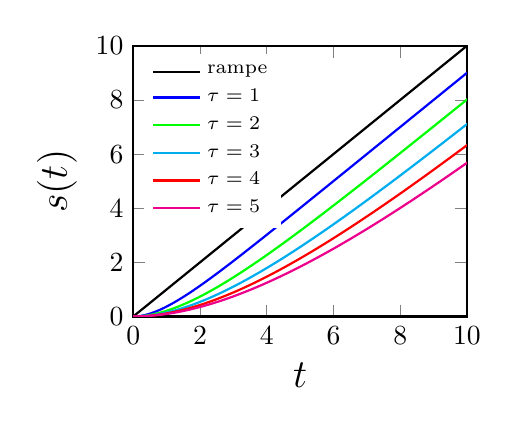
\begin{tikzpicture}
\begin{axis}[%
    legend style={draw=none,font=\scriptsize},
    legend pos=north west,
    axis line style = thick,
    width=0.48\textwidth,
    xmin=0,
    xmax=10,
    ymin=0,
    ymax=10,
    xlabel={$t$},
    ylabel={$s(t)$},
    label style={font=\Large},
    legend cell align={left},
]%
\addplot[thick,color=black,domain=0:11.5, samples=101,unbounded coords=jump]{x};
\addplot[thick,color=blue,domain=0:11.5, samples=101,unbounded coords=jump]{x-(1-exp(-x))};
\addplot[thick,color=green,domain=0:11.5, samples=101,unbounded coords=jump]{x-2*(1-exp(-x/2))};
\addplot[thick,color=cyan,domain=0:11.5, samples=101,unbounded coords=jump]{x-3*(1-exp(-x/3))};
\addplot[thick,color=red,domain=0:11.5, samples=101,unbounded coords=jump]{x-4*(1-exp(-x/4))};
\addplot[thick,color=magenta,domain=0:11.5, samples=101,unbounded coords=jump]{x-5*(1-exp(-x/5))};
\legend{rampe,$\tau=1$,$\tau=2$,$\tau=3$,$\tau=4$,$\tau=5$}
\end{axis}%
\end{tikzpicture}%
\hfill
\tikzsetnextfilename{1er_ramp2-chap2_ext}
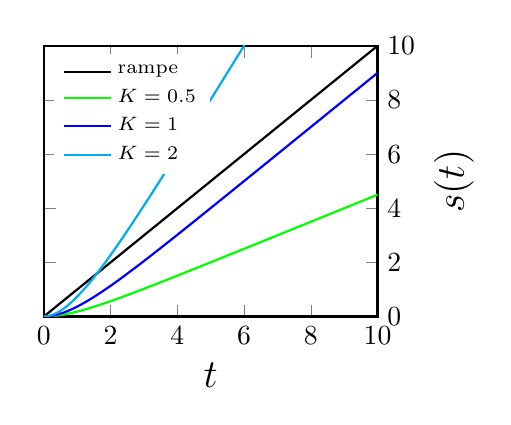
\begin{tikzpicture}
\begin{axis}[
    legend style={draw=none,font=\scriptsize},
    legend pos=north west,
    axis line style = thick,
    width=0.48\textwidth,
    xmin=0,
    xmax=10,
    ymin=0,
    ymax=10,
    xlabel={$t$},
    ylabel={$s(t)$},
    ylabel near ticks, yticklabel pos=right,
    label style={font=\Large},
    legend cell align={left},
]%
\addplot [thick,color=black,domain=0:11.5, samples=101,unbounded coords=jump]{x};
\addplot [thick,color=green,domain=0:11.5, samples=101,unbounded coords=jump]{0.5*(x-(1-exp(-x)))};
\addplot [thick,color=blue,domain=0:11.5, samples=101,unbounded coords=jump]{x-(1-exp(-x))};
\addplot [thick,color=cyan,domain=0:11.5, samples=101,unbounded coords=jump]{2*(x-(1-exp(-x)))};
\legend{rampe,$K=0.5$,$K=1$,$K=2$}
\end{axis}
\end{tikzpicture}
\caption{Réponse à une rampe d'un système du premier ordre avec $E_0=1$. (gauche) Pour différentes valeurs de $\tau$ et $K=1$ (droite) Pour différentes valeurs du gain $K$ et $\tau=1$.\label{fig-1er_ramp}}
\end{figure}
%%%%%%%%%%%%%%%%%%%%%%%%%%%%%%%%%%%%%%%%%%%%%%%%%%%%%%%%%%%%%%%%%%%%%%%%%%%%%%%%%%%%%%%
\subsubsection{Réponse à une rampe}
%%%%%%%%%%%%%%%%%%%%%%%%%%%%%%%%%%%%%%%%%%%%%%%%%%%%%%%%%%%%%%%%%%%%%%%%%%%%%%%%%%%%%%%
\index{Système du premier ordre!réponse à une rampe}
Nous considérons maitenant une excitation rampe de la forme:
$$
e(t)=E_0\cdot r(t)=E_0 t\cdot u(t) 
$$
où $E_0$ est une constante, $r(t)$ est la fonction rampe unitaire et u(t) la fonction  

La réponse à une rampe d'un système du premier ordre est, dans le domaine de Laplace,
de la forme :
$$
S(p)=H(p)E(p)=\dfrac{KE_0}{p^2(1+\tau p)}
$$

La transformée de Laplace inverse de $S(p)$ (c.f ligne 12 du tableau de l'\cref{annexe-lap}),
nous donne la forme générale de la réponse à une rampe d'un système du premier ordre:
\begin{bequation}[ams align]
    \laplacei{S(p)}=s(t)=KE_0 \left( t -\tau(1-e^{-t/\tau})\right)\label{eq-1er_ramp}  
\end{bequation}

%\begin{figure}
%\begin{center}
%\includegraphics[width=0.7\textwidth]{script/fig_1er_3.eps}
%\caption{Réponse à une rampe d'un système du premier ordre pour différentes valeurs                                        
%        de la constante de temps $\tau$  (\cref{eq-1er_ramp}) avec $K=1$ et $E_0=1$ \label{fig-1er_ramp}}
%\end{center}
%\end{figure}

La pente à l'origine peut être obtenue directement en dérivant la réponse temporelle $s(t)$. On constate 
alors que $s'(0)=0$ quelque soit $\tau$. 
À la limite $t\to\infty$ la réponse à une rampe tend vers $t-\tau$.


\newpage
%%%%%%%%%%%%%%%%%%%%%%%%%%%%%%%%%%%%%%%%%%%%%%%%%%%%%%%%%%%%%%%%%%%%%%%%%%%%%%%%%%%%%%%
\section{Système du second ordre}
%%%%%%%%%%%%%%%%%%%%%%%%%%%%%%%%%%%%%%%%%%%%%%%%%%%%%%%%%%%%%%%%%%%%%%%%%%%%%%%%%%%%%%%

%%%%%%%%%%%%%%%%%%%%%%%%%%%%%%%%%%%%%%%%%%%%%%%%%%%%%%%%%%%%%%%%%%%%%%%%%%%%%%%%%%%%%%%
\subsection{Définition d'un système du second ordre}
%%%%%%%%%%%%%%%%%%%%%%%%%%%%%%%%%%%%%%%%%%%%%%%%%%%%%%%%%%%%%%%%%%%%%%%%%%%%%%%%%%%%%%%
\index{Système du second ordre!définition}
Un système du second ordre est un système régit par une équation 
différentielle du second ordre de forme générale :
$$
\devi{s(t)}{2}+2\xi\omega_0\devi{s(t)}{}+\omega^2_0s(t)=K\omega^2_0e(t)
$$
où $\xi>0$ est le coefficient d'amortissement, $K$ le gain statique et $\omega_0>0$  
la pulsation propre du système. Cette pulsation est celle de l'oscillateur harmonique équivalent 
sans amortissement ($\xi=0$).

%%%%%%%%%%%%%%%%%%%%%%%%%%%%%%%%%%%%%%%%%%%%%%%%%%%%%%%%%%%%%%%%%%%%%%%%%%%%%%%%%%%%%%%
\subsection{Fonction de transfert d'un système du second ordre}
%%%%%%%%%%%%%%%%%%%%%%%%%%%%%%%%%%%%%%%%%%%%%%%%%%%%%%%%%%%%%%%%%%%%%%%%%%%%%%%%%%%%%%%
\index{Système du second ordre!fonction de transfert}
La transformée de Laplace de l'équation différentielle est, lorsque les CI sont toutes nulles :
$$
S(p)\left(p^2+2\xi\omega_0p+\omega^2_0\right)=K\omega^2_0E(p).
$$
La fonction de transfert $H(p)$ de ce système est donc donnée par :
\begin{bequation}[ams align]
    H(p)=\dfrac{S(p)}{E(p)}=\dfrac{K\omega^2_0}{p^2+2\xi\omega_0 p+\omega^2_0}\label{eq-2nd_ft}
\end{bequation}
La forme suivante, pour laquelle on a factorisée par $\omega^2_0$, est également très courante:
$$
H(p)=\dfrac{K}{\left(\dfrac{p}{\omega_0}\right)^2+\dfrac{2\xi p}{\omega_0}+1}
$$

%%%%%%%%%%%%%%%%%%%%%%%%%%%%%%%%%%%%%%%%%%%%%%%%%%%%%%%%%%%%%%%%%%%%%%%%%%%%%%%%%%%%%%%
\subsection{Pôles de la fonction de transfert du second ordre}
%%%%%%%%%%%%%%%%%%%%%%%%%%%%%%%%%%%%%%%%%%%%%%%%%%%%%%%%%%%%%%%%%%%%%%%%%%%%%%%%%%%%%%%
Les pôles de la fonction de transfert sont donnés par les racines du polynôme :
$$
p^2+2\xi\omega_0p+\omega_0^2 = 0
$$
le discriminant de ce polynôme est :
$$
\Delta=4\xi^2\omega^2_0-4\omega_0^2=4\omega_0^2(\xi^2-1)
$$

Les racines de ce polynôme dépendent donc du signe de $\Delta$ et ainsi de la valeur 
du taux d'amortissement $\xi$ définissant les différents régimes d'un système du second ordre :
\begin{itemize}
    \item Régime apériodique pour $\xi>1$
    \item Régime apériodique critique pour $\xi=1$
    \item Régime pseudo-périodique pour $0<\xi<1$
\end{itemize}
à noter que le cas $\xi=0$ correspond à un régime périodique associé à l'oscillateur harmonique 
au cas de l'oscillateur harmonique.
Le cas $\xi<0$ correspond à un cas divergent par définition (instable) et ne sera donc pas traité.

Le~\cref{tab-poles_2nd} résume les différents types de pôles rencontrées dans les différents régimes
du système du second ordre.

\begin{table}[!h]
    \begin{center}
\resizebox{\textwidth}{!}{
    \begin{tabular}{M{4cm}M{4.0cm}M{8.0cm}N}
        \hhline{===}
            Régime                     & Pôles   & Carte des pôles  & \\[1.5em]
        \hline
        Régime apériodique$$\xi>1$$     & Deux pôles réels $$p_{1,2}=-\xi\omega_0\pm\omega_0\sqrt{\xi^2-1}$$         &  
        \begin{center}
        \tikzsetnextfilename{2nd_pole1-chap2_ext}
        \begin{tikzpicture}
            \draw[very thick,-latex] (0,-1.5) -- (0,2.0) node[left] {Im};
            \draw[very thick,-latex] (-2.5,0) -- (1.0,0) node[below] {Re};
            \node at (-0.5,0) [thick,cross=5pt,blue] {};
            \node at (-0.5,0) [blue,below,yshift=-0.5em]     {$p_1$};
            \node at (-1.5,0) [thick,cross=5pt,blue] {};
            \node at (-1.5,0) [blue,below,yshift=-0.5em]     {$p_2$};
        \end{tikzpicture}
        \end{center} &\\ [1.5em]
        \hline
        Régime apériodique critique $$\xi=1$$ & Un pôle double réel$$p_1=p_2=-\omega_0$$ & 
        \begin{center}
        \tikzsetnextfilename{2nd_pole2-chap2_ext}
        \begin{tikzpicture}
            \draw[very thick,-latex] (0,-1.5) -- (0,2.0) node[left] {Im};
            \draw[very thick,-latex] (-2.5,0) -- (1.0,0) node[below] {Re};
            \draw[red,thick] (0,0) circle [radius=1.5];
            \draw[red,thick] (0,0) -- (-0.74999999999999967,1.299038105676658) node[midway,xshift=-1em] {$\omega_0$}; 
            \node at (-1.5,0) [thick,cross=5pt,blue] {};
            \node at (-1.5,0) [blue,below,yshift=-0.5em]     {$p_1=p_2$};
        \end{tikzpicture} 
        \end{center} &\\ [1.5em]
        \hline
        Régime pseudo-périodique $$0<\xi<1$$ & Deux pôles complexes conjugués 
        $$p_{1,2}=-\alpha\pm j\omega_d$$         
        avec $\alpha=\xi\omega_0$ et $\omega_d=\omega_0\sqrt{1-\xi^2}$ &
        \tikzsetnextfilename{2nd_pole3-chap2_ext}
        \begin{tikzpicture}
            \coordinate (o) at (0.0,0.0);
            \coordinate (p1) at (-1.0,1.0);
            \coordinate (p2) at (-1.0,-1.0);
            \draw[very thick,-latex] (0,-1.5) -- (0,2.0) coordinate (im2)  node(im) [left] {Im};
            \draw[very thick,-latex] (-2.5,0) -- (1.0,0) node(re) [below] {Re};
            \draw[blue,very thick,dotted] (p1) -- (p2) node[blue,midway,xshift=-1em,yshift=-0.8em] {$-\alpha$};
            \draw[very thick] (o) -- (p1) ;
            \draw[very thick] (o) -- (p2) ;
            \draw[red,very thick,dotted] (p1) --(0.0,1.0)   node[blue,xshift=1.2em,yshift=0em] {$\omega_d$} ;
            \draw[red,very thick,dotted] (p2) -- (0.0,-1.0) node[blue,xshift=1.2em,yshift=0em] {$-\omega_d$};
            \draw[red,thick] (0,0) circle [radius=1.41421356237];
            \node at (p1) [thick,cross=5pt,blue] {};
            \node at (p1) [blue,left,xshift=-0.5em]     {$p_1$};
            \node at (p2) [thick,cross=5pt,blue] {};
            \node at (p2) [blue,left,xshift=-0.5em]     {$p_2$};
            \pic [draw, -latex, "$\phi$", angle radius=0.5cm , angle eccentricity=1.5] {angle = im2--o--p1};
            %\pic [draw, ->, "$\phi$", angle eccentricity=1.5] {angle = p2--o--im};
        \end{tikzpicture}   &\\ [1.5em]
%        \end{center} &\\ [1.5em]
        \hhline{===}
    \end{tabular}
}
    \end{center}
    \caption{Pôles de la fonction de transfert d'un système du second ordre 
    selon le régime associé à l'amortissement.\label{tab-poles_2nd}}
\end{table}
Quelque soit le régime du système du second ordre, on peut écrire la fonction de transfert de la façon suivante en 
utilsant les pôles appropriés:
$$
H(p)=\dfrac{K\omega^2_0}{(p-p_1)(p-p_2)}
$$
Nous remarquerons également que le produit $p_1p_2=\omega^2_0$ quelque soit le régime du système, cette relation 
nous sera très utile pour l'établissement des réponses temporelles des différents régimes.

%%%%%%%%%%%%%%%%%%%%%%%%%%%%%%%%%%%%%%%%%%%%%%%%%%%%%%%%%%%%%%%%%%%%%%%%%%%%%%%%%%%%%%%
\subsection{Réponses temporelles d'un système du second ordre}
%%%%%%%%%%%%%%%%%%%%%%%%%%%%%%%%%%%%%%%%%%%%%%%%%%%%%%%%%%%%%%%%%%%%%%%%%%%%%%%%%%%%%%%
Nous allons ici, comme dans le cas des systèmes du premier ordre données les formes analytiques des
réponses temporelles (impulsionnelle, indicielle et rampe) des systèmes du second ordre.
On trouvera les réprésentations graphiques de ces réponses temporelles à l'\cref{annexe-2nd}.
%%%%%%%%%%%%%%%%%%%%%%%%%%%%%%%%%%%%%%%%%%%%%%%%%%%%%%%%%%%%%%%%%%%%%%%%%%%%%%%%%%%%%%%
\subsubsection{Réponse impulsionnelle}
%%%%%%%%%%%%%%%%%%%%%%%%%%%%%%%%%%%%%%%%%%%%%%%%%%%%%%%%%%%%%%%%%%%%%%%%%%%%%%%%%%%%%%%
\index{Système du second ordre!réponse impulsionnelle}

La réponse impulsionnelle d'un système du second ordre est, dans le domaine de Laplace, donnée 
par :
$$
S(p)=\dfrac{K\omega_0^2}{p^2+2\xi\omega_0p+\omega_0^2}
$$
où $E(p)=1$ dans le cas d'une impulsion de Dirac unitaire\footnote{Nous avons ici posé $E_0=1$ pour alléger la 
notation.}.

\'Etudions la forme analytique des réponses impulsionnelles dans les différents 
régimes du système du second ordre. 
Nous rappellons que l'étude de la réponse impulsionnelle revient à étudier la fonction de transfert du système. 

%%%%%%%%%%%%%%%%%%%%%%%%%%%%%%%%%%%%%%%%%%%%%%%%%%%%%%%%%%%%%%%%%%%%%%%%%%%%%%%%%%%%%%%
\paragraph{Dans le cas $\xi>1$ (régime apériodique),}
%%%%%%%%%%%%%%%%%%%%%%%%%%%%%%%%%%%%%%%%%%%%%%%%%%%%%%%%%%%%%%%%%%%%%%%%%%%%%%%%%%%%%%%
la sortie dans le domaine de Laplace s'écrit :
$$
S(p)=\dfrac{K\omega^2_0}{(p-p_1)(p-p_2)}
$$
La transformée de Laplace inverse de $S(p)$ (c.f ligne 16 du tableau de l'\cref{annexe-lap}),
nous donne la forme générale de la réponse impulsionnelle d'un système du second ordre en régime apériodique:

\begin{bequation}[ams align]
    s(t)&=\dfrac{K\omega^2_0}{p_1-p_2}\left(e^{p_1t}-e^{p_2t}\right) 
\end{bequation}
les exponentielles étant sans unité, les pôles sont d'unité d'inverse d'un temps,
posons donc $p_1=-1/\tau_1$ et $p_2=-1/\tau_2$, la réponse devient :
\begin{bequation}[ams align]
    s(t)&=\dfrac{K}{\tau_1-\tau_2}\left(e^{-\frac{t}{\tau_1}}-e^{-\frac{t}{\tau_2}}\right)\label{eq-1-1_2nd}
\end{bequation}

les paramètres $\tau_1$ et $\tau_2$ peuvent être considérés comme les constante de temps 
de deux systèmes du premier ordre fictifs placés en série:

\begin{center}
        \tikzsetnextfilename{2nd_sb_imp-chap2_ext}
\begin{tikzpicture}
    \sbEntree{E}
    \sbBloc[3]{H1}{$\dfrac{K_1}{1+\tau_1 p}$}{E}
        \sbRelier[$E(p)$]{E}{H1}
        \sbBloc[3]{H2}{$\dfrac{K_2}{1+\tau_2 p}$}{H1}
        \sbRelier[$X(p)$]{H1}{H2}
    \sbSortie[3]{S}{H2}
        \sbRelier[$S(p)$]{H2}{S}
\end{tikzpicture}
\end{center}
où $K_1K_2=K$.
Dans le régime apériodique un système du second ordre sera toujours considérer 
comme la mise en cascade de deux systèmes du premier ordre.

%%%%%%%%%%%%%%%%%%%%%%%%%%%%%%%%%%%%%%%%%%%%%%%%%%%%%%%%%%%%%%%%%%%%%%%%%%%%%%%%%%%%%%%
\paragraph{Dans le cas $\xi=1$ (régime apériodique critique),}
%%%%%%%%%%%%%%%%%%%%%%%%%%%%%%%%%%%%%%%%%%%%%%%%%%%%%%%%%%%%%%%%%%%%%%%%%%%%%%%%%%%%%%%
la sortie dans le domaine de Laplace s'écrit :                                                                            
$$                                                                                                                            
S(p)=\dfrac{K\omega^2_0}{(p-p_1)^2}
$$ 
La transformée de Laplace inverse de $S(p)$ (c.f ligne 8 du tableau de l'\cref{annexe-lap}),
nous donne la forme générale de la réponse impulsionnelle d'un système du second ordre en régime apériodique critique:
\begin{bequation}[ams align]
    s(t)=K\omega^2_0te^{p_1t}
\end{bequation}
posons $p_1=-1/\tau$, la réponse devient :
\begin{bequation}[ams align]
    s(t)=K\omega^2_0 t e^{-\frac{t}{\tau}}\label{eq-1-2_2nd} 
\end{bequation}


%%%%%%%%%%%%%%%%%%%%%%%%%%%%%%%%%%%%%%%%%%%%%%%%%%%%%%%%%%%%%%%%%%%%%%%%%%%%%%%%%%%%%%%
\paragraph{Dans le cas $0<\xi<1$ (régime pseudo-périodique),}
%%%%%%%%%%%%%%%%%%%%%%%%%%%%%%%%%%%%%%%%%%%%%%%%%%%%%%%%%%%%%%%%%%%%%%%%%%%%%%%%%%%%%%%
la sortie dans le domaine de Laplace s'écrit :
$$
S(p)=\dfrac{K\omega^2_0}{(p-p_1)(p-p_2)} = \dfrac{\omega^2_0}{(p+\xi\omega_0-j\omega_0\sqrt{1-\xi^2})(p+\xi\omega_0+j\omega_0\sqrt{1-\xi^2})}
$$
en posant $\alpha=\xi\omega_0$ et $\omega_d=\omega_0\sqrt{1-\xi^2}$, la sortie $S(p)$ devient :
$$
S(p)=\dfrac{K\omega^2_0}{(p+\alpha-j\omega_d)(p+\alpha+j\omega_d)} = 
     \dfrac{K\omega^2_0}{(p+\alpha)^2+\omega^2_d}=
     \dfrac{K\omega_d}{1-\xi^2}\cdot\dfrac{\omega_d}{(p+\alpha)^2+\omega^2_d}
$$
La transformée de Laplace inverse de $S(p)$ (c.f ligne 30 du tableau de l'\cref{annexe-lap}), 
nous donne la forme générale de la réponse impulsionnelle d'un système du second ordre en régime pseudo-périodique :  
\begin{bequation}[ams align]
    s(t)=\dfrac{K\omega_d}{1-\xi^2}e^{-\xi\omega_0 t}\sin{\omega_d t}\label{eq-1-3_2nd} 
\end{bequation}

%%%%%%%%%%%%%%%%%%%%%%%%%%%%%%%%%%%%%%%%%%%%%%%%%%%%%%%%%%%%%%%%%%%%%%%%%%%%%%%%%%%%%%%
\subsubsection{Réponse indicielle}
%%%%%%%%%%%%%%%%%%%%%%%%%%%%%%%%%%%%%%%%%%%%%%%%%%%%%%%%%%%%%%%%%%%%%%%%%%%%%%%%%%%%%%%
\index{Système du second ordre!réponse indicielle}
La réponse indicielle d'un système du second ordre est, dans le domaine de Laplace, donnée par :
$$
S(p)=\dfrac{K\omega_0^2}{p^2+2\xi\omega_0p+\omega_0^2}\cdot\dfrac{E_0}{p}
$$
où $E(p)=\dfrac{E_0}{p}$ est une entrée échelon.


\'Etudions la forme analytique des réponses indicielles dans les différents 
régimes du système du second ordre. 

%%%%%%%%%%%%%%%%%%%%%%%%%%%%%%%%%%%%%%%%%%%%%%%%%%%%%%%%%%%%%%%%%%%%%%%%%%%%%%%%%%%%%%%
\paragraph{Dans le cas $\xi>1$ (régime apériodique),} la sortie dans le domaine de Laplace s'écrit :
%%%%%%%%%%%%%%%%%%%%%%%%%%%%%%%%%%%%%%%%%%%%%%%%%%%%%%%%%%%%%%%%%%%%%%%%%%%%%%%%%%%%%%%
$$
S(p)=\dfrac{K\omega^2_0}{(p-p_1)(p-p_2)}\cdot\dfrac{E_0}{p}
$$
La transformée de Laplace inverse de $S(p)$ (c.f ligne 19 du tableau de l'\cref{annexe-lap}),                
nous donne la forme générale de la réponse indicielle d'un système du second ordre en régime apériodique:
%$$
%s(t)=\dfrac{KE_0\omega^2_0}{p_1p_2}\left(1+\dfrac{1}{p_1-p_2}(p_2e^{p_1t}-p_1e^{p_2t})\right)
%$$
%et en réarrangant les termes : 
\begin{bequation}[ams align]
%    s(t)&=\dfrac{\omega^2_0}{p_1p_2}\left(1+\dfrac{1}{p_1-p_2}(p_2e^{p_1t}-p_1e^{p_2t})\right)\\
    s(t)&=KE_0\left(1+\dfrac{1}{p_1-p_2}\left(p_2e^{p_1t}-p_1e^{p_2t}\right)\right)
\end{bequation}
posons $p_1=-1/\tau_1$ et $p_2=-1/\tau_2$, la réponse devient :
\begin{bequation}[ams align]
    s(t)=KE_0\left(1+\dfrac{1}{\tau_1-\tau_2}\left(\tau_2e^{-\frac{t}{\tau_2}}-\tau_1e^{-\frac{t}{\tau_1}}\right)\label{eq-2-1_2nd}\right) 
\end{bequation}
Nous pouvons à nouveau envisager cette réponse comme la réponse de deux systèmes du premier 
ordre en série.

%%%%%%%%%%%%%%%%%%%%%%%%%%%%%%%%%%%%%%%%%%%%%%%%%%%%%%%%%%%%%%%%%%%%%%%%%%%%%%%%%%%%%%%
\paragraph{Dans le cas $\xi=1$ (régime apériodique critique),} 
la sortie dans le domaine de Laplace s'écrit :
%%%%%%%%%%%%%%%%%%%%%%%%%%%%%%%%%%%%%%%%%%%%%%%%%%%%%%%%%%%%%%%%%%%%%%%%%%%%%%%%%%%%%%%
$$
S(p)=\dfrac{K\omega^2_0}{(p-p_1)^2}\cdot\dfrac{E_0}{p}
$$
La transformée de Laplace inverse de $S(p)$ (c.f ligne 14 du tableau de l'\cref{annexe-lap}),                
nous donne la forme générale de la réponse indicielle d'un système du second ordre en régime apériodique critique:
$$
s(t)=\dfrac{KE_0\omega^2_0}{p^2_1}\left(1-(1-p_1t)e^{p_1t}\right)
$$
\begin{bequation}[ams align]
    s(t)=KE_0\left(1-e^{p_1t}+p_1te^{p_1t}\right)
\end{bequation}
en posant $p_1=-\dfrac{1}{\tau}$, on obtient:
\begin{bequation}[ams align]
    s(t)=KE_0\left(1-e^{-\frac{t}{\tau}}-\dfrac{t}{\tau}e^{-\frac{t}{\tau}}\right)\label{eq-2-2_2nd} 
\end{bequation}

%%%%%%%%%%%%%%%%%%%%%%%%%%%%%%%%%%%%%%%%%%%%%%%%%%%%%%%%%%%%%%%%%%%%%%%%%%%%%%%%%%%%%%%
\paragraph{Dans le cas $0<\xi<1$ (régime pseudo-périodique),} 
la sortie $S(p)$ dans le domaine de Laplace s'écrit :
%%%%%%%%%%%%%%%%%%%%%%%%%%%%%%%%%%%%%%%%%%%%%%%%%%%%%%%%%%%%%%%%%%%%%%%%%%%%%%%%%%%%%%%
%$$
%S(p)=\dfrac{\omega^2_0}{(p-p_1)(p-p_2)}\cdot\dfrac{1}{p} = \dfrac{\omega^2_0}{(p-\xi\omega_0-j\omega_0\sqrt{1-\xi^2})(p-\xi\omega_0+j\omega_0\sqrt{1-\xi^2})}\cdot\dfrac{1}{p}
%$$
%en posant $\alpha=\xi\omega_0$ et $\omega_d=\omega_0\sqrt{1-\xi^2}$ ,$S(p)$ devient :
%$$
%S(p)=\dfrac{\omega^2_0}{(p-\alpha-j\omega_d)(p-\alpha+j\omega_d)}\cdot\dfrac{1}{p} = \dfrac{\omega^2_0}{(p-\alpha)^2+\omega^2_d}\cdot\dfrac{1}{p}
%$$
$$
S(p)=\dfrac{K\omega^2_0}{(p+\alpha)^2+\omega^2_d}\cdot\dfrac{E_0}{p}
$$
où l'on a posé $\alpha=\xi\omega_0$ et $\omega_d=\omega_0\sqrt{1-\xi^2}$.

Décomposons $S(p)$ en éléments simples,
$$
S(p)=\dfrac{A}{p} + \dfrac{B(p+\alpha)+C}{(p+\alpha)^2+\omega^2_d}
$$
procédons par évaluation pour $A$:
$$
A=pS(p)\Big|_{p=0}=\dfrac{KE_0\omega^2_0}{\alpha^2+\omega^2_d}=KE_0
$$

et identification pour B et C :
\begin{align*}
    &KE_0((p+\alpha)^2+\omega^2_d) + Bp^2+\alpha Bp+Cp = KE_0\omega^2_0 \\
    \iff & KE_0p^2+2KE_0\alpha p+KE_0(\alpha^2+\omega^2_d) + Bp^2+\alpha Bp+Cp = KE_0\omega^2_0 \\ 
\iff & 
\begin{cases}
      B+KE_0 = 0 \\ 
      2KE_0\alpha+\alpha B+C=0
\end{cases} \\
\iff & \begin{cases}
      B=-KE_0     \\
      C=-KE_0\alpha
  \end{cases}
\end{align*}

on obtient alors :
\begin{align*}
    S(p)&=KE_0\left(\dfrac{1}{p} - \dfrac{(p+\alpha)}{(p+\alpha)^2+\omega^2_d} - \dfrac{\alpha}{(p+\alpha)^2+\omega^2_d}\right) \\
    S(p)&=KE_0\left(\dfrac{1}{p} - \dfrac{(p+\alpha)}{(p+\alpha)^2+\omega^2_d} - \dfrac{\xi}{\sqrt{1-\xi^2}} \dfrac{\omega_d}{(p+\alpha)^2+\omega^2_d}\right)
\end{align*}

La transformée de Laplace inverse de $S(p)$ (c.f lignes 3, 30 et 31 du tableau de l'\cref{annexe-lap}),                
nous permet de déterminer la réponse indicielle :
\begin{align*}
    s(t) &= KE_0\left(1 - e^{-\alpha t}\cos{(\omega_d t)} - \dfrac{\xi}{\sqrt{1-\xi^2}} e^{-\alpha t}\sin{(\omega_d t)}\right) \\
    s(t) &= KE_0\left( 1- \dfrac{1}{\sqrt{1-\xi^2}} e^{-\alpha t}\left ( \sqrt{1-\xi^2}\cos{(\omega_d t)} + \xi\sin{(\omega_d t)}\right)\right) \\
\end{align*}
en posant : 
\begin{align*}
    \cos{\phi}&=\xi\\
    \sin{\phi}&=\sqrt{1-\xi^2}
\end{align*}
on obtient :
$$
s(t) = KE_0 \left( 1- \dfrac{1}{\sqrt{1-\xi^2}} e^{-\alpha t}\left ( \sin{\phi}\cos{(\omega_d t)} + \cos\phi\sin{(\omega_d t)}\right) \right)
$$
et enfin la forme générale de la réponse indicielle d'un système du second ordre en régime pseudo-périodique s'écrit :
\begin{bequation}[ams align]
    s(t) = KE_0 \left( 1 - \dfrac{1}{\sqrt{1-\xi^2}} e^{-\xi\omega_0 t}\sin{(\omega_d t+\phi)}\right)\label{eq-2-3_2nd} 
\end{bequation}

\begin{figure}[!t]
\begin{center}
        \tikzsetnextfilename{2nd_pp-chap2_ext}
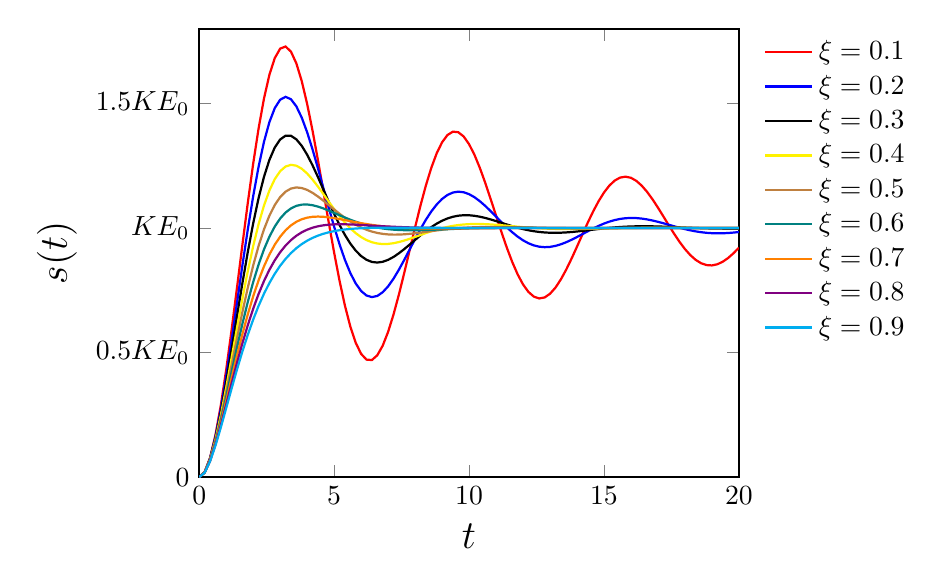
\begin{tikzpicture}
        \begin{axis}[
        legend style={draw=none},
        %legend pos={east outer},
        legend pos=outer north east,
        axis line style = thick,
        xmin=0,
        xmax=20,
        ymin=0,
        ymax=1.8,
        xlabel={$t$},
        ylabel={$s(t)$},
        ytick={0,0.5,1,1.5},
        yticklabels={0,$0.5KE_0$,$KE_0$,$1.5KE_0$},
        label style={font=\Large},
        cycle list name=color list,
        ]
    \def\a{0.1}
    \def\b{0.99}
    \def\w{0.994987437107}
    \def\p{1.47062890563}
    \addplot+[thick,domain=0:20, samples=101,unbounded coords=jump]{1-((1./\w)*exp(-\a*x)*sin(deg(x)*\w+deg(\p)))};

    \def\a{0.2}
    \def\b{0.96}
    \def\w{0.979795897113}
    \def\p{1.369438406}
    \addplot+[thick,domain=0:20, samples=101,unbounded coords=jump]{1-((1./\w)*exp(-\a*x)*sin(deg(x)*\w+deg(\p)))};

    \def\a{0.3}
    \def\b{0.91}
    \def\w{0.953939201417}
    \def\p{1.26610367278}
    \addplot+[thick,domain=0:20, samples=101,unbounded coords=jump]{1-((1./\w)*exp(-\a*x)*sin(deg(x)*\w+deg(\p)))};

    \def\a{0.4}
    \def\b{0.84}
    \def\w{0.916515138991}
    \def\p{1.15927948073}
    \addplot+[thick,domain=0:20, samples=101,unbounded coords=jump]{1-((1./\w)*exp(-\a*x)*sin(deg(x)*\w+deg(\p)))};
    
    \def\a{0.5}
    \def\b{0.75}
    \def\w{0.866025403784}
    \def\p{1.0471975512}
    \addplot+[thick,domain=0:20, samples=101,unbounded coords=jump]{1-((1./\w)*exp(-\a*x)*sin(deg(x)*\w+deg(\p)))};

    \def\a{0.6}
    \def\b{0.64}
    \def\w{0.8}
    \def\p{0.927295218002}
    \addplot+[thick,domain=0:20, samples=101,unbounded coords=jump]{1-((1./\w)*exp(-\a*x)*sin(deg(x)*\w+deg(\p)))};

    \def\a{0.7}
    \def\b{0.51}
    \def\w{0.714142842854}
    \def\p{0.795398830184}
    \addplot+[thick,domain=0:20, samples=101,unbounded coords=jump]{1-((1./\w)*exp(-\a*x)*sin(deg(x)*\w+deg(\p)))};

    \def\a{0.8}
    \def\b{0.3599999999999999}
    \def\w{0.6}
    \def\p{0.643501108793}
    \addplot+[thick,domain=0:20, samples=101,unbounded coords=jump]{1-((1./\w)*exp(-\a*x)*sin(deg(x)*\w+deg(\p)))};

    \def\a{0.9}
    \def\b{0.18999999999999995}
    \def\w{0.435889894354}
    \def\p{0.451026811796}
    \addplot+[thick,domain=0:20, samples=101,unbounded coords=jump]{1-((1./\w)*exp(-\a*x)*sin(deg(x)*\w+deg(\p)))};

    \legend{$\xi=0.1$,$\xi=0.2$, $\xi=0.3$, $\xi=0.4$, $\xi=0.5$, $\xi=0.6$, $\xi=0.7$, $\xi=0.8$, $\xi=0.9$} 
\end{axis}
\end{tikzpicture}
\caption{Réponse indicielle d'un système du second ordre en régime pseudo-périodique pour 
différentes valeurs du taux d'amortissement $\xi$  (??\Cref{eq-1er_ramp}) avec $\omega_0=1$. \label{fig-2nd_pp}}
\end{center}
\end{figure}

Il est maintenant possible d'interpréter les différentes grandeurs introduites. En effet,
cette réponse a la forme d'une sinuso\"ide de pulsation $\omega_d$
(dite pseudo-pulsation), de phase $\phi$ et amortie par une exponentielle décroissante dépendant de $\xi$.
La~\cref{fig-2nd_pp} présente cette réponse indicielle du régime pseudo-périodique pour différentes valeurs du 
taux d'amortissement pour une pulsation propre $\omega_0=1$.
Nous constatons que comme attendu, l'amplitude des oscillations augmente lorsque le taux d'amortissement diminue.

\newpage
%%%%%%%%%%%%%%%%%%%%%%%%%%%%%%%%%%%%%%%%%%%%%%%%%%%%%%%%%%%%%%%%%%%%%%%%%%%%%%%%%%%%%%%%%%%%%%%%%%%
\paragraph{Dépassement et temps de réponse à 5\%}
%%%%%%%%%%%%%%%%%%%%%%%%%%%%%%%%%%%%%%%%%%%%%%%%%%%%%%%%%%%%%%%%%%%%%%%%%%%%%%%%%%%%%%%%%%%%%%%%%%%
Certaines propriétés de la réponse indicielle dans le régime pseudo-périodique sont fortement 
dépendantes du taux d'amortissement. C'est le cas du dépassemement et du temps de réponse. 
La~\cref{fig-2nd_depassement_1} présente la réponse à un échelon unitaire pour un amortissement de $\xi=0.2$, 
on observe que les dépassements succésifs sont de moins en moins important. Pour déterminer la relation entre
le dépassement et le taux d'amortissement, il nous faut d'abord déterminer le temps du premier maximum $t_1$.

\begin{figure}[!h]
\begin{center}
        \tikzsetnextfilename{2nd_depassement_1-chap2_ext}
    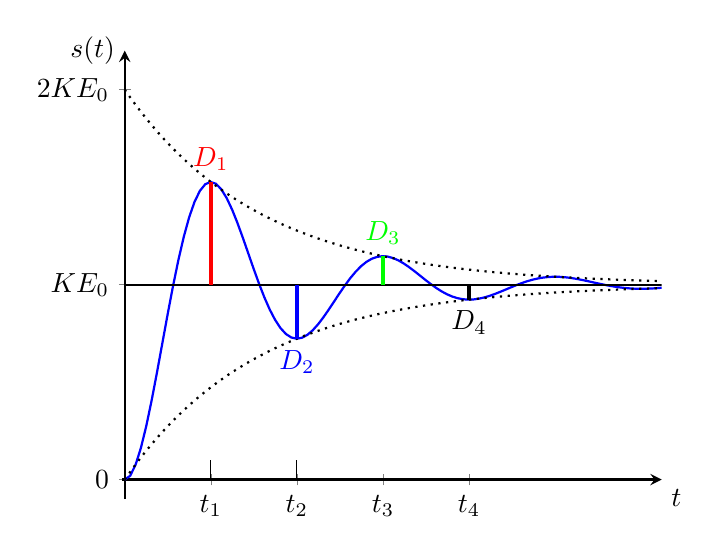
\begin{tikzpicture}
        \pgfmathsetmacro{\a}{0.2}             % amortissement xi
        \pgfmathsetmacro{\b}{0.96}            % 1-xi^2 
        \pgfmathsetmacro{\w}{0.979795897113}  % w_d=w_0 sqrt(1-xi^2)
        \pgfmathsetmacro{\p}{1.369438406}     % phi =arctan(xi/1-xi^2)
        \pgfmathsetmacro{\tu}{3.206374575405548}    % t1 = 
        \pgfmathsetmacro{\td}{6.4127491508093204}   % t2 = 2*t1
        \pgfmathsetmacro{\ttt}{9.619123726213981}    % t3 = 3*t1
        \pgfmathsetmacro{\tq}{12.82549830161864}    % t4 = 4*t1
        \pgfmathsetmacro{\du}{1.526620599330303}     % dépassement d1 
        \pgfmathsetmacro{\dd}{0.72267074436099255}     % dépassement d2 
        \pgfmathsetmacro{\dt}{1.146047298816441}     % dépassement d3 
        \pgfmathsetmacro{\dq}{0.92308848396671406}     % dépassement d4 

        %>>> 1+np.exp(-0.2*np.pi/np.sqrt((1-0.2*0.2)))+1
        %>>> 1-np.exp(-2*0.2*np.pi/np.sqrt((1-0.2*0.2)))+1
        %>>> 1+np.exp(-3*0.2*np.pi/np.sqrt((1-0.2*0.2)))+1
        %>>> 1-np.exp(-4*0.2*np.pi/np.sqrt((1-0.2*0.2)))+1
        %1.526620599330303
        %0.72267074436099255
        %1.146047298816441
        %0.92308848396671406

        \begin{axis}[
        %ticks=none,
        axis line style = thick,
        %height=9cm,
        %width=12cm,
        axis x line=center,
        axis y line=center,
        xmin=-0.1,
        xmax=20,
        ymin=-0.1,
        ymax=2.2,
        xlabel={$t$},
        ylabel={$s(t)$},
        xlabel style={below right},
        ylabel style={left},
        xticklabels={$t_1$,$t_2$,$t_3$,$t_4$},
        xtick={\tu,\td,\ttt,\tq},
        yticklabels={0,$KE_0$,$2KE_0$},
        ytick={0.001,1,2}
        ]
        \addplot [thick,color=blue,domain=0:20, samples=101,unbounded coords=jump]{1-((1./\w)*exp(-\a*x)*sin(deg(x)*\w+deg(\p)))};
        \addplot [thick,dotted,domain=0:20, samples=101,unbounded coords=jump]{1+exp(-\a*x)};
        \addplot [thick,dotted,domain=0:20, samples=101,unbounded coords=jump]{1-exp(-\a*x)};
        \addplot [thick,domain=0:20, samples=101,unbounded coords=jump]{1};
            \draw [ultra thick, red] (axis cs:\tu,1)  -- (axis cs:\tu,\du) node[above] {$D_1$};
            \draw [ultra thick, blue] (axis cs:\td,1)  -- (axis cs:\td,\dd) node[below] {$D_2$};
            \draw [ultra thick, green] (axis cs:\ttt,1) -- (axis cs:\ttt,\dt) node[above] {$D_3$};
            \draw [ultra thick, black] (axis cs:\tq,1)  -- (axis cs:\tq,\dq) node[below] {$D_4$};
            \draw (axis cs:\tu,0) -- (axis cs:\tu,0.1);
            \draw (axis cs:\td,0) -- (axis cs:\td,0.1);
        \end{axis}
    \end{tikzpicture}
\end{center}
    \caption{Définition du dépassement observé dans le cas de la réponse indicielle en régime pseudo-périodique 
    d'un système du second ordre. Les deux enveloppes correspondent aux exponentielles
    décroissantes $1+e^{-\alpha t}$ et $1-e^{-\alpha t}$. \label{fig-2nd_depassement_1}}
\end{figure}

\begin{figure}[!h]
\begin{center}
        \tikzsetnextfilename{2nd_depassement_2-chap2_ext}
        \begin{tikzpicture}
    \pgfplotsset{signaltmp/.style={signaln,domain=0.0001:1,
                              unbounded coords=jump}
                }
    \pgfmathsetmacro{\pi}{3.141592653589793}     % dépassement d4 
    \begin{axis}
    [   xmode=log,
        ymode=log,
        width=0.65\textwidth,
        axis line style = thick,
        xmin=0.01,
        xmax=1,
        ymin=0.01,
        ymax=1.0,
        xlabel={$\xi$},
        ylabel={$D_k$},
        label style={font=\Large},
        grid=both,
        grid style={line width=.4pt, draw=black},
        major grid style={line width=.4pt,draw=black},
        legend style={draw=none,font=\normalsize},
        legend pos=outer north east,
        label style={font=\Large},
        legend cell align={left},
    ]
    \addplot[signaltmp,vtcol1] {exp(-(x*\pi)/(sqrt(1-x*x)))};
    \addplot[signaltmp,vtcol2] {exp(-(2*x*\pi)/(sqrt(1-x*x)))};
    \addplot[signaltmp,vtcol3] {exp(-(3*x*\pi)/(sqrt(1-x*x)))};
    \addplot[signaltmp,vtcol4] {exp(-(4*x*\pi)/(sqrt(1-x*x)))};
    \legend{$k=1$,$k=2$,$k=3$,$k=4$}
    \end{axis}
\end{tikzpicture}


\caption{Variation de la valeur $D_k$ du k-ème dépassement en fonction du taux 
    d'amortissement $\xi$. \label{fig-2nd_depassement_2}}
\end{center}
\end{figure}

Pour celà il suffit de déterminer le temps pour lequel la dérivée du signal $s(t)$ s'annule. On
calcul alors un temps $t_1$ à $T_d/2$ où $T_d$ est la 
pseudo-période définit à partir de la pseudo-pulsation $\omega_d$. 
On a alors :
\begin{align*}
T_d=\dfrac{2\pi}{\omega_d}\\
t_1 = \dfrac{\pi}{\omega_d}
\end{align*}

Formellement, le premier dépassement est définit par :
$$
D_1=\left|\dfrac{s(t_1)-s(\infty)}{s(\infty)-s(0)}\right|
$$
où $s(0)$, $s(\infty)$ et $s(t_1)$ sont respectivement la valeur initiale, la valeur finale et la valeur du premier 
maximum du signal.

La valeur $s(t_1)$ s'obtient en remplaçant la valeur de $t_1$ dans la forme analytique de la réponse 
indicielle du régime pseudo-périodique (\Cref{eq-2-3_2nd}) :
\begin{align*}
    s(t_1) &= KE_0\left(1 - \dfrac{1}{\sqrt{1-\xi^2}} e^{-\alpha t_1}\sin{(\omega_d t_1+\phi)}\right) \\
    s(t_1) &= KE_0\left(1 - \dfrac{1}{\sqrt{1-\xi^2}} e^{-\alpha\pi/\omega_d}\sin{(\pi+\phi)}\right) \\
    s(t_1) &= KE_0\left(1 + e^{-\alpha\pi/\omega_d}\right)
\end{align*}
Le dépassement est donc donné par l'expression : 
\begin{bequation}[ams align]
    D=e^{-\dfrac{\xi\pi}{\sqrt{1-\xi^2}}}
\end{bequation}
et le $k$-ème dépassement $D_k$ est lui donné par :
\begin{bequation}[ams align]
    D_k=e^{-\dfrac{k\xi\pi}{\sqrt{1-\xi^2}}}
\end{bequation}

La~\cref{fig-2nd_depassement_2} présente cette relation entre le dépassement  et le taux d'amortissement.
Il est possible d'utiliser cette figure comme un abaque\footnote{Les abaques sont très répandus en automatique. 
Ils permettent de s'affranchir de nombreux claculs en lisant des valeurs directement sur un graphique.} 
facilitant le calcul du dépassement connaissant le taux d'amortissement et inversement.
\newline

Il n'existe pas de relation analytique simple pour déterminer 
le temps de réponse à 5\% (c.f définition donnée par la~\cref{fig-2nd_t5pc}) en fonction du taux d'amortissement. 
Nous avons alors procéder par une méthode numérique, qui pourra constituer un exercice de travaux pratiques  
sous Scilab (\Cref{annexe-scilab}). 
La~\cref{fig-2nd_temps_reponse} présente la variation du temps de réponse à 5\% réduit 
à la pulsation (i.e $\omega_0\cdot t_{5\%}$ ) en fonction du taux d'amortissement $\xi$. On observe un minimum du 
temps de réponse pour $\xi\sim 0.7$

\begin{figure}[!h]
\begin{center}
    \tikzsetnextfilename{2nd_t5pc-chap2_ext}
    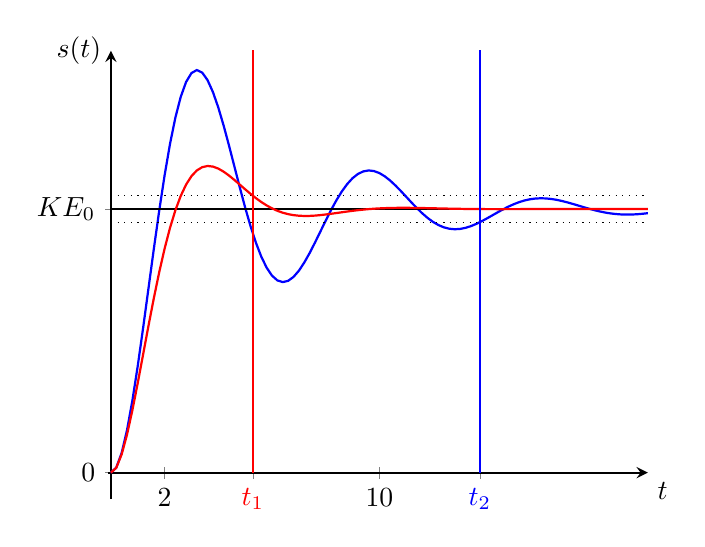
\begin{tikzpicture}
        \pgfmathsetmacro{\a}{0.2}             % amortissement xi
        \pgfmathsetmacro{\b}{0.96}            % 1-xi^2 
        \pgfmathsetmacro{\w}{0.979795897113}  % w_d=w_0 sqrt(1-xi^2)
        \pgfmathsetmacro{\p}{1.369438406}     % phi =arctan(xi/1-xi^2)

        \begin{axis}[
            axis line style = thick,
            %height=8cm,
            %width=12cm,
            axis x line=center,
            axis y line=center,
            xmin=-0.1,
            xmax=20,
            ymin=-0.1,
            ymax=1.6,
            xlabel={$t$},
            ylabel={$s(t)$},
            xlabel style={below right},
            ylabel style={left},
            xticklabels={2,\textcolor{red}{$t_1$},10,\textcolor{blue}{$t_2$}},
            xtick={2,5.29,10,13.74},
            yticklabels={0,$KE_0$,2},
            ytick={0.001,1,2}
                    ]
        \addplot [thick,color=blue,domain=0:20, samples=101,unbounded coords=jump]{1-((1./\w)*exp(-\a*x)*sin(deg(x)*\w+deg(\p)))};
        \addplot [thick,domain=0:20, samples=101,unbounded coords=jump]{1};
        \addplot [dotted,domain=0:20, samples=101,unbounded coords=jump]{1.05};
        \addplot [dotted,domain=0:20, samples=101,unbounded coords=jump]{0.95};
        
        \def\a{0.5}
        \def\b{0.75}
        \def\w{0.866025403784}
        \def\p{1.0471975512}
        \addplot [thick,domain=0:20, color=red,samples=101,unbounded coords=jump]{1-((1./\w)*exp(-\a*x)*sin(deg(x)*\w+deg(\p)))};
        \draw[blue,thick] (axis cs:13.74,0) -- (axis cs:13.74,2);
        \draw[red,thick] (axis cs:5.29,0) -- (axis cs:5.29,2);
        \end{axis}
    \end{tikzpicture}
\end{center}
    \caption{Définition du temps de réponse à 5\% dans le cas de la réponse indicielle en régime pseudo-périodique 
    d'un système du second ordre. Le temps de réponse à 5\% est définit comme le temps minimal 
    pour que le signal soit compris dans une bande à $\pm$5\% autour de la valeur finale. Réponse indicielle 
    pour (bleu) $\xi=0.2$ et (rouge) $\xi=0.5$.\label{fig-2nd_t5pc} }
\end{figure}

\begin{figure}
\centering
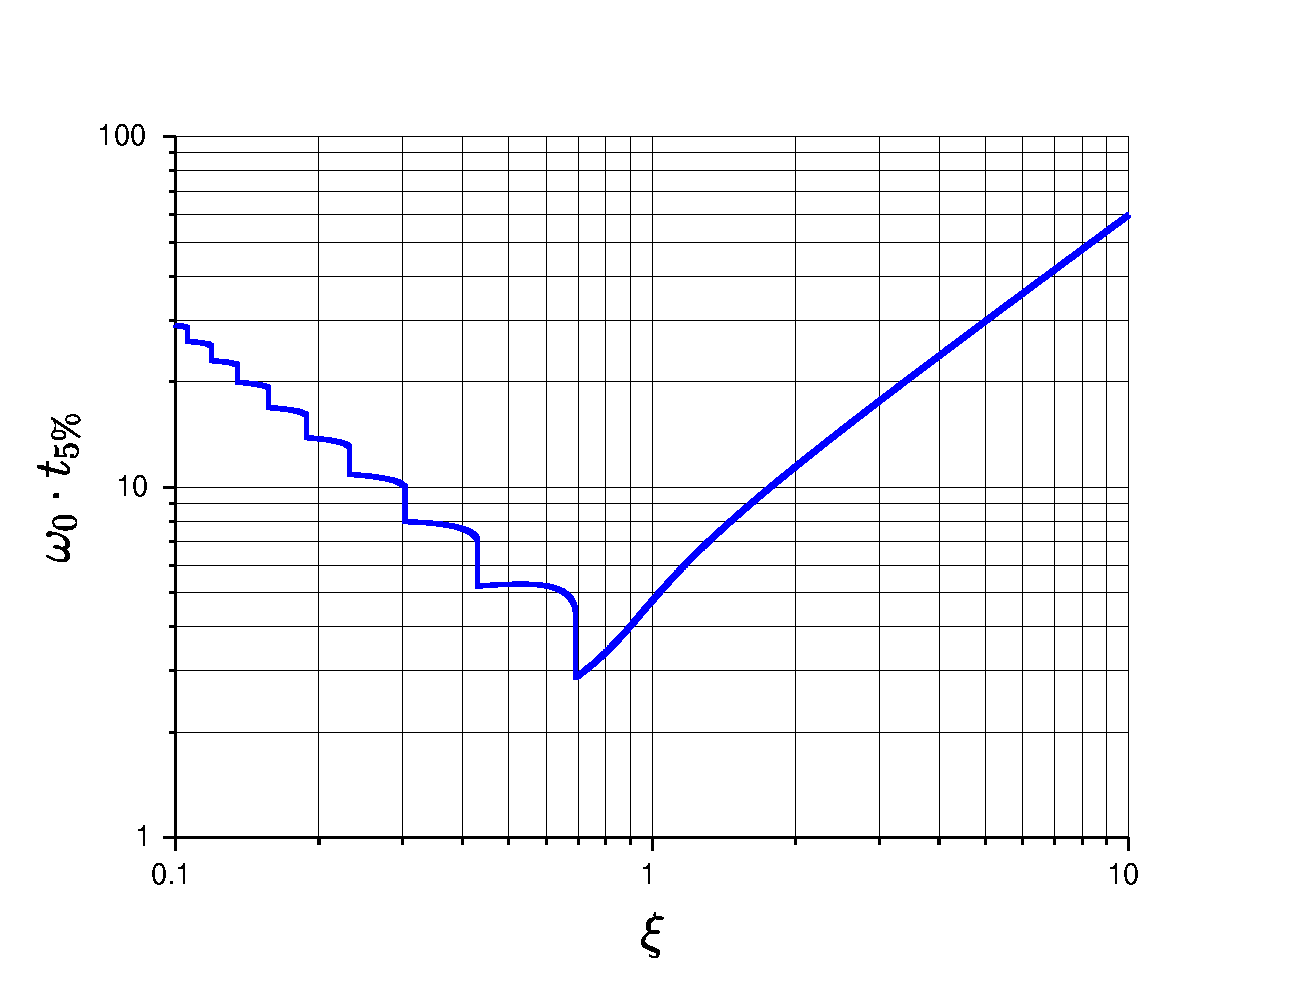
\includegraphics[width=0.7\textwidth]{scilab/fig_temps_de_reduit.eps}
    \caption{Temps de réponse à 5\% réduit en fonction du taux d'amortissement $\xi$. 
     Le minimum est atteint pour $\xi\sim0.7$ pour lequel $\omega_0\cdot t_{5\%}\sim3$.\label{fig-2nd_temps_reponse}}
\end{figure}


\newcommand{\mysize}{\footnotesize}
\resizebox{\textwidth}{!}{
        \begin{tabular}{M{2.75cm}M{5.25cm}M{5.25cm}M{5.25cm}}%
        \hhline{====}
             Réponse   & Régime apérodique        ($\xi>1$)  & Régime critique ($\xi=1$) & 
                         Régime pseudo-périodique ($0<\xi<1$) \\[0em]
        \hline
        Réponse impulsionnelle & 
            \resizebox{0.9\linewidth}{!}{\begin{tikzpicture}
    \begin{axis}
    [   legend style={draw=none},
        axis line style = thick,
        xmin=0,
        xmax=12,
        ymin=0,
        ymax=0.3,
        xlabel={$t$},
        ylabel={$s(t)$},
        label style={font=\Large},
        grid=both,
        grid style={line width=.4pt, draw=black},
        major grid style={line width=.4pt,draw=black},
    ]
    \addplot[signalb,domain=0:12] {(1/(3.73-0.26))*exp(-x/3.73)-exp(-x/0.26)};
    \end{axis}
\end{tikzpicture}
} 
            {\mysize $$ s(t)=\dfrac{1}{\tau_1-\tau_2}\left(e^{-\frac{t}{\tau_1}}-e^{-\frac{t}{\tau_2}}\right)$$} &  
            \resizebox{0.9\linewidth}{!}{    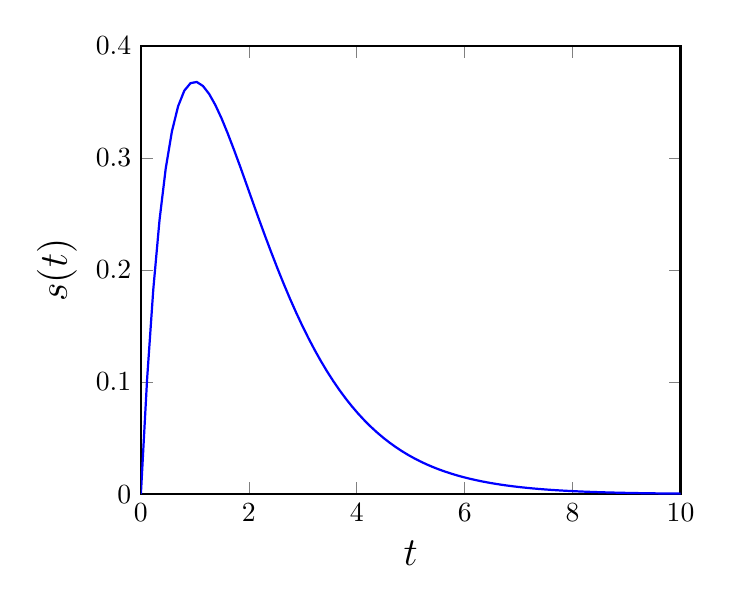
\begin{tikzpicture}
        \begin{axis}[
        legend style={draw=none},
        axis line style = thick,
        xmin=0,
        xmax=10,
        ymin=0,
        ymax=0.4,
        xlabel={$t$},
        ylabel={$s(t)$},
        label style={font=\Large},
        ]
            \addplot [thick,color=blue,domain=0:11.5, samples=101,unbounded coords=jump]{x*exp(-x)};
        \end{axis}
    \end{tikzpicture}
} 
            {\mysize $$s(t)=\dfrac{t}{\tau^2}e^{-\frac{t}{\tau}}$$} &  
            \resizebox{0.9\linewidth}{!}{\tikzsetnextfilename{2nd_rep_1_3_ext}
\begin{tikzpicture}
    \begin{axis}
    [   legend style={draw=none},
        axis line style = thick,
        xmin=0,
        xmax=12,
        ymin=-0.6,
        ymax=1.2,
        xlabel={$t$},
        ylabel={$s(t)$},
        label style={font=\Large},
        grid=both,
        grid style={line width=.4pt, draw=black},
        major grid style={line width=.4pt,draw=black},
    ]
    \def\a{0.3}            
    \def\b{0.91}           
    \def\w{0.953939201417} 
    \addplot[signalb,domain=0:12] {(\w/\b)*exp(-\a*x)*sin(deg(x)*\w)};
    \end{axis}
\end{tikzpicture}
} 
            {\mysize $$s(t)=\dfrac{\omega_d}{1-\xi^2}e^{-\xi\omega_0 t}\sin{\omega_d t}$$}\\[0em]
        \hline
        Réponse indicielle &  
            \resizebox{0.9\linewidth}{!}{\tikzsetnextfilename{2nd_rep_2_1_ext}
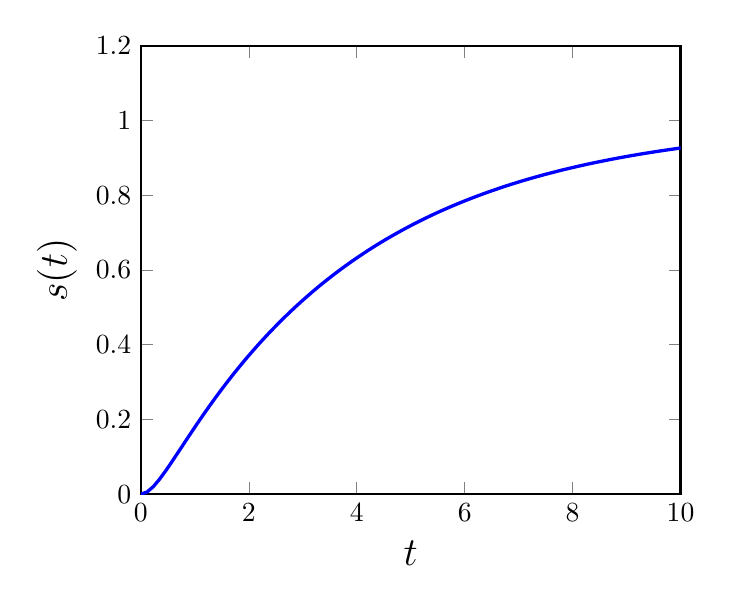
\begin{tikzpicture}
    \def\tu{2.0}
    \def\td{1.0}
    \begin{axis}
    [   legend style={draw=none},
        axis line style = thick,
        xmin=0,
        xmax=10,
        ymin=0,
        ymax=1.2,
        xlabel={$t$},
        ylabel={$s(t)$},
        label style={font=\Large},
    ]
    \addplot[very thick,color=blue,domain=0:11.5, samples=101]
    {1+(1/(3.73-0.26))*(0.26*exp(-x/0.26)-3.73*exp(-x/3.73))};
    \end{axis}
\end{tikzpicture}
} 
            {\mysize $$s(t)=1+\dfrac{1}{\tau_1-\tau_2}\left(\tau_2e^{-\frac{t}{\tau_2}}-\tau_1e^{-\frac{t}{\tau_1}}\right)$$} &  
            \resizebox{0.9\linewidth}{!}{\begin{tikzpicture}
    \begin{axis}
    [   legend style={draw=none},
        axis line style = thick,
        xmin=0,
        xmax=10,
        ymin=0,
        ymax=1.2,
        xlabel={$t$},
        ylabel={$s(t)$},
        label style={font=\Large},
        grid=both,
        grid style={line width=.4pt, draw=black},
        major grid style={line width=.4pt,draw=black},
    ]
    \addplot[signalb,domain=0:10]  {1-exp(-x)-x*exp(-x)};
    \end{axis}
\end{tikzpicture}
} 
            {\mysize $$s(t)=1-e^{-\frac{t}{\tau}}-\dfrac{t}{\tau}e^{-\frac{t}{\tau}}$$ } &  
            \resizebox{0.9\linewidth}{!}{\tikzsetnextfilename{2nd_rep_2_3_ext}
\begin{tikzpicture}
\begin{axis}
[   
    legend style={draw=none},
    axis line style = thick,
    xmin=0,
    xmax=12,
    ymin=0,
    ymax=1.5,
    xlabel={$t$},
    ylabel={$s(t)$},
    label style={font=\Large},
    grid=both,
    grid style={line width=.4pt, draw=black},
    major grid style={line width=.4pt,draw=black},
]
\def\a{0.3}            
\def\b{0.91}           
\def\w{0.954} 
\def\p{1.266}  
\addplot[signalb,domain=0:12] {1-((1./\w)*exp(-\a*x)*sin(deg(x)*\w+deg(\p)))};
\end{axis}
\end{tikzpicture}
} 
            {\mysize $$s(t) = 1 - \dfrac{e^{-\xi\omega_0 t}}{\sqrt{1-\xi^2}}\sin{(\omega_d t+\phi)}$$}\\[0em]
        \hhline{====}
        \end{tabular}
}



%%%%%%%%%%%%%%%%%%%%%%%%%%%%%%%%%%%%%%%%%%%%%%%%%%
\subsubsection{Réponse à une rampe}
%%%%%%%%%%%%%%%%%%%%%%%%%%%%%%%%%%%%%%%%%%%%%%%%%%
\index{Système du second ordre!réponse à une rampe}
La réponse à une rampe d'un système du second ordre est, dans le domaine de Laplace, donnée par
$$
S(p)=\dfrac{K\omega_0^2}{p^2+2\xi\omega_0p+\omega_0^2}\cdot\dfrac{E_0}{p^2}
$$
où $E(p)=\dfrac{E_0}{p^2}$ est un signal rampe.
\'Etudions la forme analytique des réponses à une rampe dans les différents régimes du système du second ordre.

%%%%%%%%%%%%%%%%%%%%%%%%%%%%%%%%%%%%%%%%%%%%%%%%%%%%%%%%%%%%%%%%%%%%%%%%%%%%%%%%%%%%%%%
\paragraph{Dans le cas $\xi>1$ (régime apériodique),}
%%%%%%%%%%%%%%%%%%%%%%%%%%%%%%%%%%%%%%%%%%%%%%%%%%%%%%%%%%%%%%%%%%%%%%%%%%%%%%%%%%%%%%%
écrivons la sortie $S(p)$ sous la forme :
$$
S(p)=\dfrac{K\omega_0^2}{(p-p_1)(p-p_2)}\cdot\dfrac{E_0}{p^2}
$$
la décomposition en éléments simples de $S(p)$ s'écrit:
$$
S(p)=\dfrac{A}{p}+\dfrac{B}{p^2}+\dfrac{C}{p-p_1}+\dfrac{D}{p-p_2}.
$$
Procédons par évaluation pour obtenir les coefficients $B$, $C$ et $D$:
\begin{align*}
    B=p^2S(p)\Big|_{p=0}      &=KE_0,\\
    C=(p-p_1)S(p)\Big|_{p=p_1}&=\dfrac{KE_0\omega_0^2}{p_1^2(p_1-p_2)}=\dfrac{KE_0 p_2^2}{\omega_0^2(p_1-p_2)},\\
    D=(p-p_2)S(p)\Big|_{p=p_2}&=\dfrac{KE_0\omega_0^2}{p_2^2(p_2-p_1)}=\dfrac{-KE_0 p_1^2}{\omega_0^2(p_1-p_2)},
\end{align*}
et par indentification pour $A$:
$$
A=KE_0\dfrac{p_1+p_2}{\omega_0^2}
$$
la sortie $S(p)$ devient alors :
$$
S(p)=KE_0\left(\dfrac{p_1+p_2}{\omega_0^2}\cdot\dfrac{1}{p} + \dfrac{1}{p^2} +\dfrac{1}{\omega_0^2(p_1-p_2)}\left(\dfrac{p_2^2}{p-p_1}-\dfrac{p_1^2}{p-p_2} \right) \right)
$$
La transformée de Laplace inverse de $S(p)$ (c.f lignes 4 et 7 du tableau de l'\cref{annexe-lap}),                
nous permet de déterminer la réponse à une rampe du régime apériodique :
\begin{bequation}[ams align]
    s(t)=KE_0\left(t+\dfrac{p_1+p_2}{\omega_0^2}+\dfrac{1}{\omega_0^2(p_1-p_2)}\left(p_2^2e^{p_1t}-p_1^2e^{p_2t}\right)\right)
\end{bequation}
posons $p_1=-1/\tau_1$ et $p_2=-1/\tau_2$, la réponse devient :
\begin{bequation}[ams align]
    s(t)=KE_0\left(t-\tau_1-\tau_2+\dfrac{1}{(\tau_1-\tau_2)}\left(\tau_1^2e^{-\frac{t}{\tau_1}}-\tau_2^2e^{-\frac{t}{\tau_2}}\right)\right)
\end{bequation}
%%%%%%%%%%%%%%%%%%%%%%%%%%%%%%%%%%%%%%%%%%%%%%%%%%%%%%%%%%%%%%%%%%%%%%%%%%%%%%%%%%%%%%%
\paragraph{Dans le cas $\xi=1$ (régime apériodique critique),} 
%%%%%%%%%%%%%%%%%%%%%%%%%%%%%%%%%%%%%%%%%%%%%%%%%%%%%%%%%%%%%%%%%%%%%%%%%%%%%%%%%%%%%%%
écrivons la sortie $S(p)$ sous la forme :
$$
S(p)=\dfrac{K\omega_0^2}{(p-p_1)^2}\cdot\dfrac{E_0}{p^2}.
$$
La décomposition en éléments simples de $S(p)$ s'écrit:
$$                                                                                                                            
S(p)=\dfrac{A}{p}+\dfrac{B}{p^2}+\dfrac{C}{(p-p_1)}+\dfrac{D}{(p-p_1)^2}.
$$ 
Procédons par évaluation pour obtenir les coefficients $B$ et $D$:
\begin{align*}
    B=p^2S(p)\Big|_{p=0}        &=KE_0,\\
    D=(p-p_1)^2S(p)\Big|_{p=p_1}&=KE_0,\\
\end{align*}
par identification on obtient:
$$
A=KE_0\dfrac{2}{p_1}
$$
et en utilisant la parité de la fonction $C=-A$.

La sortie $S(p)$ devient alors :
$$                                                                                                                            
S(p)=KE_0\left(\dfrac{2}{p_1}\cdot\dfrac{1}{p}+ \dfrac{1}{p^2} - \dfrac{2}{p_1}\cdot\dfrac{1}{(p-p_1)}+ \dfrac{1}{(p-p_1)^2}\right)  
$$ 
La transformée de Laplace inverse de $S(p)$ (c.f lignes 3, 4, 7 et 8 du tableau de l'\cref{annexe-lap}), 
nous permet de déterminer la réponse à une rampe du régime apériodique critique :
\begin{bequation}[ams align]
    s(t)=KE_0\left(\dfrac{2}{p_1}+t-\dfrac{2}{p_1}e^{p_1t}+te^{p_1t}\right)
\end{bequation}
posons $p_1=-1/\tau$, la réponse devient :
\begin{bequation}[ams align]
    s(t)=KE_0(t-2\tau+(t+2\tau)e^{-\frac{t}{\tau}})
\end{bequation}

%%%%%%%%%%%%%%%%%%%%%%%%%%%%%%%%%%%%%%%%%%%%%%%%%%%%%%%%%%%%%%%%%%%%%%%%%%%%%%%%%%%%%%%
\paragraph{Dans le cas $0<\xi<1$ (régime pseudo-périodique),} 
%%%%%%%%%%%%%%%%%%%%%%%%%%%%%%%%%%%%%%%%%%%%%%%%%%%%%%%%%%%%%%%%%%%%%%%%%%%%%%%%%%%%%%%
écrivons la sortie $S(p)$ sous la forme:
$$
S(p)=\dfrac{K\omega_0^2}{(p+\alpha)^2+\omega_d^2}\cdot\dfrac{E_0}{p^2},
$$
où, rappellons que $\alpha=\xi\omega_0$ et $\omega_d=\omega_0\sqrt{1-\xi^2}$.

La décomposition en éléments simples de $S(p)$ s'écrit:
$$                                                                                                                            
S(p)=\dfrac{A}{p}+\dfrac{B}{p^2}+\dfrac{C(p+\alpha)+D}{(p+\alpha)^2+\omega_d^2}.
$$ 
Procédons par évaluation pour obtenir le coefficient $B$:
$$
B=p^2S(p)\Big|_{p=0}=\dfrac{KE_0\omega_0^2}{\alpha^2+\omega_d^2}=KE_0,
$$
où $\alpha^2+\omega_d^2=\omega_0^2$ par définition.

Par identification du numérateur,
%\begin{align*}
%Ap\left((p+\alpha)^2+\omega_d^2\right)+B\left((p+\alpha)^2+\omega_d^2\right)+Cp^2(p+\alpha)+Dp^2=KE_0\omega_0^2\\
%Ap(p^2+2p\alpha+\alpha^2+\omega_d^2)+B(p^2+2p\alpha+\alpha^2+\omega_d^2)+Cp^3+Cp^2\alpha+Dp^2=KE_0\omega_0^2\\
%    Ap^3+2Ap^2\alpha+Ap(\alpha^2+\omega_d^2)+Bp^2+2Bp\alpha+B(\alpha^2+\omega_d^2)+Cp^3+Cp^2\alpha+Dp^2=KE_0\omega_0^2\\
%    p^3(A+C)+p^2(2A\alpha+B+C\alpha+D)+p(A(\alpha^2+\omega_d^2)+2B\alpha)+B(\alpha^2+\omega_d^2)=KE_0\omega_0^2\\
%\end{align*}
on obtient les relations suivantes sur les coefficients:
$$
\begin{cases}
    p^3:\,\,\,\,\,A+C=0\\
    p^2:\,\,\,\,\,B+2A\alpha+C\alpha+D=0\\
    p^1:\,\,\,\,\,2B\alpha+A(\alpha^2+\omega_d^2)=0
\end{cases}
$$
On a alors :
\begin{align*}
    A=-\dfrac{2\alpha}{\alpha^2+\omega_d^2}B&=-\dfrac{2\xi}{\omega_0}KE_0\\
    C=-A&=\dfrac{2\xi}{\omega_0}KE_0\\
    D=-B-A\alpha&=KE_0\left(\dfrac{2\xi}{\omega_0}\alpha-1\right)=KE_0(2\xi^2-1)
\end{align*}
La sortie $S(p)$ s'écrit donc :
$$
S(p)=KE_0\left(\dfrac{1}{p^2}-\dfrac{2\xi}{\omega_0}\cdot\dfrac{1}{p}+\dfrac{2\xi}{\omega_0}\cdot\dfrac{p+\alpha}{(p+\alpha)^2+\omega_d^2} + \dfrac{2\xi^2-1}{\omega_d}\cdot\dfrac{\omega_d}{(p+\alpha)^2+\omega_d^2}\right)
$$
La transformée de Laplace inverse de $S(p)$ (c.f lignes 3, 4, 30 et 31 du tableau de l'\cref{annexe-lap}),         
nous permet de déterminer la réponse à une rampe du régime pseudo-périodique :
\begin{align*}
    s(t)=KE_0\left(t-\dfrac{2\xi}{\omega_0}+\dfrac{2\xi\sqrt{1-\xi^2}}{\omega_d}e^{-\alpha t}\cos{\omega_d t}+\dfrac{2\xi^2-1}{\omega_d}e^{-\alpha t}\sin{\omega_d t}\right)\\
%    s(t)=KE_0\left(t-\dfrac{2\xi}{\omega_0}+\dfrac{2\xi}{\omega_d}e^{-\alpha t}\left(\sqrt{1-\xi^2}\cos{\omega_d t}+\xi\sin{\omega_d t}\right)-\dfrac{1}{\omega_d}e^{-\alpha t}\sin{\omega_d t}\right)\\
\end{align*}
en posant à nouveau : 
\begin{align*}
    \cos{\phi}&=\xi\\
    \sin{\phi}&=\sqrt{1-\xi^2}
\end{align*}
et en notant que :
\begin{align*}
    \cos{2\phi}&=1-2\sin^2\phi=2\xi^2-1\\
    \sin{2\phi}&=2\sin\phi\cos\phi=2\xi\sqrt{1-\xi^2}
\end{align*}

on obtient :
\begin{bequation}[ams align]
s(t)=KE_0\left(t-\dfrac{2\xi}{\omega_0}+\dfrac{2\xi}{\omega_d}e^{-\alpha t}\sin{(\omega_d t+2\phi)}\right)
\end{bequation}

\begin{figure}[!t]
\begin{center}
        \tikzsetnextfilename{2nd_ramp-chap2_ext}
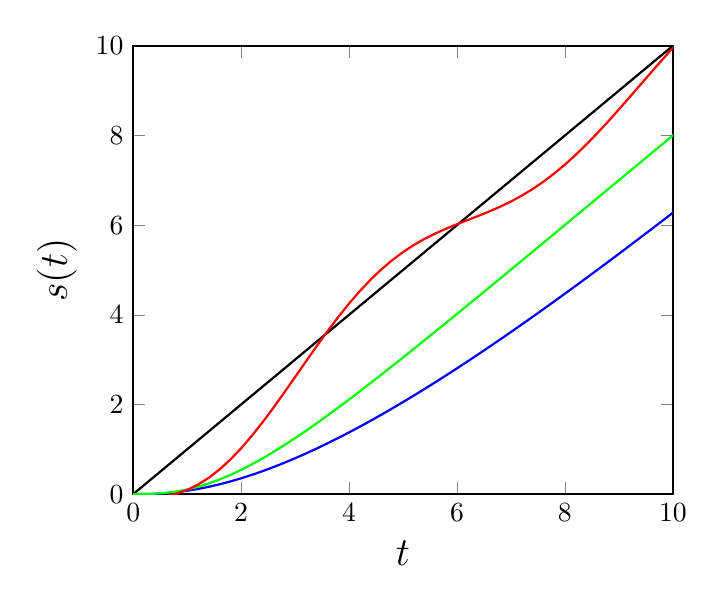
\begin{tikzpicture}
\begin{axis}[
        legend style={draw=none},
        legend pos=outer north east,
        axis line style = thick,
        xmin=0,
        xmax=10,
        ymin=0,
        ymax=10,
        xlabel={$t$},
        ylabel={$s(t)$},
        label style={font=\Large},
        cycle list name=color list,
        ]
\addplot[thick,color=black,domain=0:10, samples=101,unbounded coords=jump]{x};
% xi=2 
\def\a{0.28867513459481292}
\def\u{3.73205080757}
\def\d{0.267949192431}
\def\us{13.928203230275509}
\def\ds{0.07179676972449088}
\addplot[thick,color=blue,domain=0:20, samples=101,unbounded coords=jump]{x+-\u-\d+\a*(\us*exp(-x/\u)-\ds*exp(-x/\d))};

\addplot[thick,color=green,domain=0:20, samples=101,unbounded coords=jump]{((x-2)+(x+2)*exp(-x))};

\def\a{0.1}
\def\b{0.99}
\def\w{0.994987437107}
\def\p{1.47062890563}

%\def\a{0.2}
%\def\b{0.96}
%\def\w{0.979795897113}
%\def\p{1.369438406}
%\def\pd{-2.73887681201}

\addplot[thick,color=red,domain=0:20, samples=101,unbounded coords=jump]{x-2*\a+\a/\w*exp(-\a*x)*sin(\w*deg(x)+deg(\p))-(1/\w)*exp(-\a*x)*sin(\w*deg(x))};
%\addplot[thick,color=gray,domain=0:20, samples=101,unbounded coords=jump]{x-2*\a+(1/\w)*exp(-\a*x)*sin(\w*deg(x)-deg(\pd))};

\end{axis}
\end{tikzpicture}
    \caption{Réponse à une rampe d'un système du second ordre en (bleu) régime apériodique avec $\xi=2.0$, (vert) régime apériodique critique (i.e $\xi=1$) et en (rouge) régime pseudo-périodique avec $\xi=0.1$. Avec $\omega_0=1$, $K=1$ et $E_0=1$. \label{fig-2nd_ramp}}
\end{center}
\end{figure}

%%%%%%%%%%%%%%%%%%%%%%%%%%%%%%%%%%%%%%%%%%%%%%%%%%%%%%%%%%%%%%%%%%%%%%%%%%%%%%%%%%%%
%%%%%%%%%%%%%%%%%%%%%%%%%%%%%%%%%%%%%%%%%%%%%%%%%%%%%%%%%%%%%%%%%%%%%%%%%%%%%%%%%%%%
\subsection{Cas particulier de l'oscillateur harmonique}
%%%%%%%%%%%%%%%%%%%%%%%%%%%%%%%%%%%%%%%%%%%%%%%%%%%%%%%%%%%%%%%%%%%%%%%%%%%%%%%%%%%%
%%%%%%%%%%%%%%%%%%%%%%%%%%%%%%%%%%%%%%%%%%%%%%%%%%%%%%%%%%%%%%%%%%%%%%%%%%%%%%%%%%%%

Dans le cas où l'équation différentielle est de la forme 
$$
\devi{s(t)}{2}+\omega_0^2 s(t)=Ke(t)
$$
c'est à dire sans amortissement ($\xi=0$), on se retrouve alors dans le 
cas classique de l'oscillateur harmonique.
Nous allons ici étudier ce modèle limite qui est d'une grande importance en physique.
Ceci afin de constater que l'approche utilisée tout le long de ce chapitre
permet également de décrire ce modèle important. 

La fonction de transfert de l'équation différentielle précédente s'écrit :
$$
H(p)=\dfrac{S(p)}{E(p)}=\dfrac{K}{p^2+\omega_o^2}
$$

%%%%%%%%%%%%%%%%%%%%%%%%%%%%%%%%%%%%%%%%%%%%%%%%%%%%%%%%%%%%%%%%%%%%%%%%%%%%%%%%%%%%%%%
\subsubsection{Réponse impulsionnelle}
%%%%%%%%%%%%%%%%%%%%%%%%%%%%%%%%%%%%%%%%%%%%%%%%%%%%%%%%%%%%%%%%%%%%%%%%%%%%%%%%%%%%%%%
La réponse impulsionnelle d'un oscillateur harmonique est, dans le domaine de Laplace,
donnée par 
$$
S(p)=\dfrac{KE_0}{p^2+\omega_o^2}
$$
La réponse dans le domaine temporelle est donnée par :
$$
s(t)=\laplace{S(p)}=\dfrac{KE_0}{\omega_0}\sin{\omega_0t}
$$
Ce qui correspond bien à l'oscillation incessante d'un oscillateur que l'on a 
déplacé de son état d'équilibre.

\newpage
%%%%%%%%%%%%%%%%%%%%%%%%%%%%%%%%%%%%%%%%%%%%%%%%%%%%%%%%%%%%%%%%%%%%%%%%%%%%%%%%%%%%
%%%%%%%%%%%%%%%%%%%%%%%%%%%%%%%%%%%%%%%%%%%%%%%%%%%%%%%%%%%%%%%%%%%%%%%%%%%%%%%%%%%%
%%%%%%%%%%%%%%%%%%%%%%%%%%%%%%%%%%%%%%%%%%%%%%%%%%%%%%%%%%%%%%%%%%%%%%%%%%%%%%%%%%%%
\section{Autres modèles particuliers}
%r%%%%%%%%%%%%%%%%%%%%%%%%%%%%%%%%%%%%%%%%%%%%%%%%%%%%%%%%%%%%%%%%%%%%%%%%%%%%%%%%%%%
%%%%%%%%%%%%%%%%%%%%%%%%%%%%%%%%%%%%%%%%%%%%%%%%%%%%%%%%%%%%%%%%%%%%%%%%%%%%%%%%%%%%
%%%%%%%%%%%%%%%%%%%%%%%%%%%%%%%%%%%%%%%%%%%%%%%%%%%%%%%%%%%%%%%%%%%%%%%%%%%%%%%%%%%%

Dans cette partie, nous allons présenter des modèles théoriques particuliers 
qui physiquement ne se retrouveront jamais seuls. Cependant ils compléteront les 
modèles du premier et second ordre discutés précedemment.

%%%%%%%%%%%%%%%%%%%%%%%%%%%%%%%%%%%%%%%%%%%%%%%%%%%%%%%%%%%%%%%%%%%%%%%%%%%%%%%%%%%%
%%%%%%%%%%%%%%%%%%%%%%%%%%%%%%%%%%%%%%%%%%%%%%%%%%%%%%%%%%%%%%%%%%%%%%%%%%%%%%%%%%%%
\subsection{Gain pur}
%%%%%%%%%%%%%%%%%%%%%%%%%%%%%%%%%%%%%%%%%%%%%%%%%%%%%%%%%%%%%%%%%%%%%%%%%%%%%%%%%%%%
%%%%%%%%%%%%%%%%%%%%%%%%%%%%%%%%%%%%%%%%%%%%%%%%%%%%%%%%%%%%%%%%%%%%%%%%%%%%%%%%%%%%
\index{Gain pur}
Dans le cas où l'équation différentielle\footnote{Bien évidemment 
dans ce cas présent, l'équation différentielle est d'ordre 0. Ce qui est 
un cas très particulier d'équation différentielle.}~régissant le système est de la forme :
$$
s(t)=Ke(t)
$$
avec $K$ un gain pur. Autrement dit, la sortie est proportionnelle à l'entrée et
de même nature.
En effet, la réponse temporelle est trivialement donné par la définition 
même du modèle, il est cependant possible de définir une fonction
de transfert qui s'écrit :
\begin{bequation}[ams align]
H(p)=\dfrac{S(p)}{E(p)}=K
\end{bequation}
La \textbf{réponse impulsionnelle} pour une entrée du type impulsion de Dirac unitaire 
est elle même une impulsion de Dirac :
$$
s(t)=K\delta(t)
$$
De même pour la \textbf{réponse indicielle} pour une entrée en échelon $e(t)=E_0u(t)$
$$
s(t)=KE_0u(t)
$$
%%%%%%%%%%%%%%%%%%%%%%%%%%%%%%%%%%%%%%%%%%%%%%%%%%%%%%%%%%%%%%%%%%%%%%%%%%%%%%%%%%%%
%%%%%%%%%%%%%%%%%%%%%%%%%%%%%%%%%%%%%%%%%%%%%%%%%%%%%%%%%%%%%%%%%%%%%%%%%%%%%%%%%%%%
\subsection{Intégrateur pur}
%%%%%%%%%%%%%%%%%%%%%%%%%%%%%%%%%%%%%%%%%%%%%%%%%%%%%%%%%%%%%%%%%%%%%%%%%%%%%%%%%%%%
%%%%%%%%%%%%%%%%%%%%%%%%%%%%%%%%%%%%%%%%%%%%%%%%%%%%%%%%%%%%%%%%%%%%%%%%%%%%%%%%%%%%
\index{Intégrateur pur}
Dans le cas où l'équation différentielle régissant le système est de la forme :
$$
\devi{s(t)}{}=Ke(t)
$$
où $K$ est un gain. La sortie correspond à l'intégrale de l'entrée :
$$
s(t)=K\int\limits_0^t e(\tau)\dd{\tau}
$$
La fonction de transfert est celle d'un intégrateur pur:
\begin{bequation}[ams align]
H(p)=\dfrac{S(p)}{E(p)}=\dfrac{K}{p}.
\end{bequation}

La \textbf{réponse impulsionnelle}, pour une entrée unitaire, est la fonction échélon unitaire:
$$
s(t)=K\int\limits_0^t \delta(\tau)\dd{\tau}=Ku(t)
$$
La  \textbf{réponse indicielle} est une rampe de pente $KE_0$ :
$$
s(t)=KE_0\int\limits_0^t u(\tau)\dd{\tau}=KE_0\left[\tau\right]_0^t=KE_0t
$$
\begin{figure}
\centering
\tikzsetnextfilename{integrateur_1-chap2_ext}
\begin{tikzpicture}
\begin{axis}[%
    name=first,
    axis line style = thick,
    width=0.49\textwidth,
    xmin=-1,
    xmax=5,
    ymin=0,
    ymax=1.2,
    xlabel={$t$},
    ylabel={$s(t)$},
    label style={font=\Large},
]%
\addplot[very thick,color=blue,domain=-1:0, samples=10,unbounded coords=jump] {{0}};
\addplot[very thick,color=blue,domain=0:11.5, samples=10,unbounded coords=jump] {{1}};
\draw[dashed,very thick,blue] (axis cs:0,0) -- (axis cs:0,1);
\draw[dblarw={black}{2pt}{2pt}] (axis cs:0,0) -- (axis cs:0,1);
\end{axis}%
\begin{axis}[
    at=(first.east),anchor=west,xshift=0.5cm,
    axis line style = thick,
    width=0.49\textwidth,
    xmin=-0.2,
    xmax=1.2,
    ymin=0,
    ymax=1.2,
    xlabel={$t$},
    ylabel={$s(t)$},
    ylabel near ticks, yticklabel pos=right,
    label style={font=\Large},
]%
\addplot[very thick,color=blue,domain=-1:0, samples=10,unbounded coords=jump]{{0}};%
\addplot[very thick,color=blue,domain=0:11.5, samples=10,unbounded coords=jump]{{x}};%
\draw[dashed,very thick,black] (axis cs:0,0) -- (axis cs:0,1);
\addplot[very thick,color=black,domain=-1:0, samples=10,unbounded coords=jump] {{0}};
\addplot[very thick,color=black,domain=0:11.5, samples=10,unbounded coords=jump] {{1}};
\end{axis}
\end{tikzpicture}
\caption{(gauche) Réponse impulsionnelle (droite) Réponse indicielle d'un intégrateur avec $K=1$ et $E_0=1$.\label{fig-integ}}
\end{figure}

Autrement dit, le système est \textbf{instable}.

%%%%%%%%%%%%%%%%%%%%%%%%%%%%%%%%%%%%%%%%%%%%%%%%%%%%%%%%%%%%%%%%%%%%%%%%%%%%%%%%%%%%
%%%%%%%%%%%%%%%%%%%%%%%%%%%%%%%%%%%%%%%%%%%%%%%%%%%%%%%%%%%%%%%%%%%%%%%%%%%%%%%%%%%%
\subsection{Dérivateur pur}
%%%%%%%%%%%%%%%%%%%%%%%%%%%%%%%%%%%%%%%%%%%%%%%%%%%%%%%%%%%%%%%%%%%%%%%%%%%%%%%%%%%%
%%%%%%%%%%%%%%%%%%%%%%%%%%%%%%%%%%%%%%%%%%%%%%%%%%%%%%%%%%%%%%%%%%%%%%%%%%%%%%%%%%%%
\index{Dérivateur pur}
Dans le cas où l'équation différentielle régissant le système est de la forme :
$$
s(t)=K\devi{e(t)}{}
$$
où $K$ est un gain. On a à faire à un système dit dérivateur pur. 
La sortie correspond alors à la dérivée de l'entrée.
Sa fonction de transfert est de la forme :
\begin{bequation}[ams align]
H(p)=\dfrac{S(p)}{E(p)}=Kp
\end{bequation}

La \textbf{réponse impulsionnelle} d'un dérivateur n'est pas définie. 
La \textbf{réponse indicielle} est une impulsion de Dirac, par définition de la dérivée d'un échelon :
$$
s(t)=K\delta(t)
$$

%%%%%%%%%%%%%%%%%%%%%%%%%%%%%%%%%%%%%%%%%%%%%%%%%%%%%%%%%%%%%%%%%%%%%%%%%%%%%%%%%%%%
%%%%%%%%%%%%%%%%%%%%%%%%%%%%%%%%%%%%%%%%%%%%%%%%%%%%%%%%%%%%%%%%%%%%%%%%%%%%%%%%%%%%
\subsection{Retard pur}
%%%%%%%%%%%%%%%%%%%%%%%%%%%%%%%%%%%%%%%%%%%%%%%%%%%%%%%%%%%%%%%%%%%%%%%%%%%%%%%%%%%%
%%%%%%%%%%%%%%%%%%%%%%%%%%%%%%%%%%%%%%%%%%%%%%%%%%%%%%%%%%%%%%%%%%%%%%%%%%%%%%%%%%%%
\index{Retard pur}
Un système retard est régit par l'équation différentielle :
$$
s(t)=e(t-\tau)
$$
Sa fonction de transfert est donc de la forme :
\begin{bequation}[ams align]
H(p)=\dfrac{S(p)}{E(p)}=Ke^{-\tau p}
\end{bequation}
Les réponses temporelles sont donc de mêmes natures que leurs solliciations, 
elles sont simplement retardés de $\tau$.

\newpage
%%%%%%%%%%%%%%%%%%%%%%%%%%%%%%%%%%%%%%%%%%%%%%%%%%%%%%%%%%%%%%%%%%%%%%%%%%%%%%%%%%%%
\section{Généralisation des modèles de SLCI}
%%%%%%%%%%%%%%%%%%%%%%%%%%%%%%%%%%%%%%%%%%%%%%%%%%%%%%%%%%%%%%%%%%%%%%%%%%%%%%%%%%%%

Nous venons d'analyser un grand nombre de systèmes d'ordre $n<2$. 
Nous allons ici généraliser l'approche pour l'étude de ssystèmes d'ordre supérieur à deux.

\subsection{Systèmes d'ordre supérieur à 2}
Dans le cas d'un système d'ordre $n>2$, il suffit de décomposée en éléments simples 
la fonction de transfert, qui n'est rien d'autre qu'une fraction rationnelle en $p$ et 
d'utiliser la propriété de linéarité de la sortie.

Rappelons (c.f ~\cref{chap-slci}) que toute fonction de transfert peut être 
mise sous la forme factorisé suivante  
$$
H(p)=\dfrac{K}{p^\alpha}\cdot\dfrac{N(p)}{D(p)}
$$
avec $K$ le gain statique, $\alpha$ la classe (ou le nombre d'intégrateur) et 
deux polynômes $N(p)$ et $D(p)$.

Les deux polynômes peuvent se factoriser comme un produit de polynômes 
irréductibles unitaires, c'est à dire :
$$
H(p)=\dfrac{K}{p^\alpha}\dfrac{\prod\limits_i (1+\tau_ip)\prod\limits_j (1+2\xi_j\tau_jp+\tau_jp^2)}{\prod\limits_i (1+\tau_ip)\prod\limits_j (1+2\xi_j\tau_jp+\tau_jp^2)}
$$
en toute rigueur il suffit d'exprimer le rapport 
des produits comme un simple produits en permettant
les exposants d'être négatifs, soit alors la forme plus condensée :
\begin{bequation}[ams align]
H(p)= Kp^{\alpha}\prod_{i} (1+\tau_ip)^{n_i}\prod_{j} (1+2\xi_j\tau_jp+\tau_jp^2)^{n_j}
\end{bequation}
où $n_i$ et $n_j$ peuvent être positifs et négatifs. 

Après décomposition en éléments simples, $H(p)$ s'écrit sous la forme d'une somme
de systèmes du 1er et second ordre.
$$
H(p)=\sum_i H_i(p)
$$
La réponse temporelle $s(t)$ d'un tel système sortie est alors la somme des réponses de
chacuns des sous systèmes $H_i(p)$
$$
s(t)=\sum_i s_i(t)
$$

\subsection{Exemple d'une fonction de transfert d'ordre 3}

Soit un système caractérisé par la fonction de transfert $H(p)$ tel
que :
$$
H(p)=\dfrac{3p+1}{p^3+9p^2+23p+15}
$$
On détermine, après un peu d'algèbre, les trois pôles 
$p_1=-1$, $p_2=-3$ et $p_3=-5$ ainsi que la forme factorisée de la fonction de transfert :
$$
H(p)=\dfrac{3p+1}{(p+1)(p+3)(p+5)}
$$

La décomposition en éléments simples est donné par :
$$
H(p)=\dfrac{0.25}{p+1}+\dfrac{1}{p+3}-\dfrac{1.25}{p+5}
$$
et sous forme factorisée :
$$
H(p)=\dfrac{0.25}{p+1}+\dfrac{1/3}{\frac{1}{3}p+1}-\dfrac{0.25}{0.2p+1}
$$

La réponse temporelles est donc la somme des réponses temporelles de trois systèmes 
du premier ordre $H_1(p)$, $H_2(p)$ et $H_3(p) $ ayant respectivement pour paramètres
($K_1=0.25$,$\tau_1=1$), ($K_2=1/3,$$\tau_2=1/3$) et ($K_3=-0.25$,$\tau_3=0.2$)

Pour la réponse indicielle à un échelon d'amplitude $E_0$ les réponses $s_i(t)$ 
de chacunes de ces fonctions de transferts sont de la forme :
$$
s_i(t)=K_iE_0\left(1-e^{-t/\tau_i}\right)
$$

La réponse indicielle du système est alors
$$
s(t)=\sum_i s_i(t) = \dfrac{E_0}{4}\left(1-e^{-t}\right)+\dfrac{E_0}{3}\left(1-e^{-3t}\right)-\dfrac{E_0}{4}\left(1-e^{-5t}\right)
$$

La valeur finale est donnée par la somme algébrique des valeurs finales de chacunes
des fonctions de transfert.

Cependant, les propriétés telle que le temps de réponse, 
les pseudo-oscillation (dans le cas de système du second ordre) 
le dépassement ou encore la stabilité sont gouvernées 
par la fonction de transfert de 
temps caractéristique le plus grand. On dit que c'est un pôle dominant.

\subsection{Notion de pôles dominants}

Soient $p_1,\ldots,p_n$ les pôles d'un système stable\footnote{À partir 
des résultats obtenus dans ce chapitre il est déjà clair que la stabilité
d'un système dépend également des pôles de sa fonction de transfert}.
Le pôle $p_i$ est dit dominant si la valeur absolue
de sa partie réelle est largement plus petite que celle de tout autre pôles 
du système\footnote{Dans la pratique un rapport de 5 est 
suffisant pour considérer une domination d'un pôle sur les autres}
\begin{bequation}[ams align]
	\big|\Re{p_i}\big| \ll \big|\Re{p_j}\big|\;\; \forall j\neq i
\end{bequation}

Pour observer l'influence d'un pôle dominant sur 
la réponse temporelle d'un système linéaire, nous
nous allons l'illustrer par l'étude d'une fonction 
de transfert du second ordre en régime apériodique.
Une telle fonction de transfert est équivalente à deux
systèmes du premier ordre en série.

Prenons l'exemple de la fonction de transfert définie par  
$$
H(p)=\dfrac{5}{(p+1)(5p+1)}
$$
et de décomposition en éléments simples telle que :
$$
H(p)=\dfrac{A}{p+1}+\dfrac{B}{5p+1}
$$
Par identification on peut écrire $H(p)$ en fonction de
deux fonctions de transferts $H_1(p)$ et $H_2(p)$ tel que :
\begin{align*}
	H(p)&=H_1(p)-H_2(p)\\
	H_1(p)&=\dfrac{6.25}{5p+1}\\
	H_2(p)&=\dfrac{1.25}{p+1}
\end{align*}

Par définition, le pôle dominant est donné par $H_1(p)$.
Pour observer son effet traçons les réponses indicielles 
de ces trois fonctions de transfert.

\begin{figure}[!h]
\begin{center}
{\tikzset{external/export=false}       
\tikzsetnextfilename{test-chap2_ext}
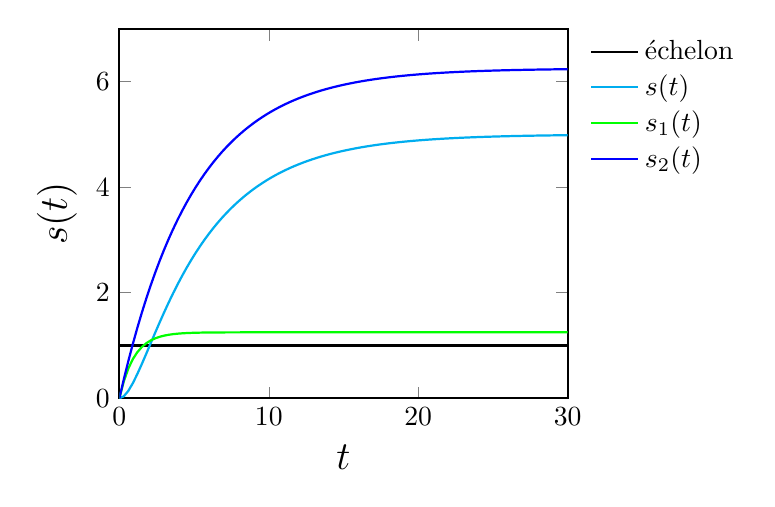
\begin{tikzpicture}
\begin{axis}[%
    legend style={draw=none,font=\normalsize},
    legend pos=outer north east,
    axis line style = thick,
    width=0.6\textwidth,
    xmin=0,
    xmax=30,
    ymin=0,
    ymax=7,
    xlabel={$t$},
    ylabel={$s(t)$},
    label style={font=\Large},
    legend cell align={left},
]%
	\addplot[thick,color=black,domain=0:30, samples=101,unbounded coords=jump] {{1}};
	\addplot[thick,color=cyan,domain=0:30, samples=101,unbounded coords=jump]{6.25*(1-exp(-x/5))-1.25*(1-exp(-x))};
	\addplot[thick,color=green,domain=0:30, samples=101,unbounded coords=jump]{1.25*(1-exp(-x))};
	\addplot[thick,color=blue,domain=0:30, samples=101,unbounded coords=jump]{6.25*(1-exp(-x/5))};
	\legend{échelon,$s(t)$,$s_1(t)$,$s_2(t)$}
\end{axis}%
\end{tikzpicture}
}
\end{center}
\caption{}
\end{figure}


\begin{center}
{\tikzset{external/export=false}       
\begin{tikzpicture}[scale=1.2]
    \carte[l]
    \dpole{-2}{0}{1}[blue]
    \dpole{-0.5}{0}{2}[blue]
\end{tikzpicture}
}
\end{center}


\newpage
%%%%%%%%%%%%%%%%%%%%%%%%%%%%%%%%%%%%%%%%%%%%%%%%%%%%%%%%%%%%%%%%%%%%%%%%%%%%%%%%%%%%
\section{Identification d'un modèle de comportement}
%%%%%%%%%%%%%%%%%%%%%%%%%%%%%%%%%%%%%%%%%%%%%%%%%%%%%%%%%%%%%%%%%%%%%%%%%%%%%%%%%%%%

\subsection{Formule de Bureau}
\acplhp

\subsection{Modèle de Strejc}
\acplhp


%\newpage
%%%%%%%%%%%%%%%%%%%%%%%%%%%%%%%%%%%%%%%%%%%%%%%%%%%%%%%%%%%%%%%%%%%%%%
%%%%%%%%%%%%%%%%%%%%%%%%%%%%%%%%%%%%%%%%%%%%%%%%%%%%%%%%%%%%%%%%%%%%%%
%%%%%%%%%%%%%%%%%%%%%%%%%%%%%%%%%%%%%%%%%%%%%%%%%%%%%%%%%%%%%%%%%%%%%%
%\section*{Exercices du chapitre}
%%%%%%%%%%%%%%%%%%%%%%%%%%%%%%%%%%%%%%%%%%%%%%%%%%%%%%%%%%%%%%%%%%%%%%
%%%%%%%%%%%%%%%%%%%%%%%%%%%%%%%%%%%%%%%%%%%%%%%%%%%%%%%%%%%%%%%%%%%%%%
%%%%%%%%%%%%%%%%%%%%%%%%%%%%%%%%%%%%%%%%%%%%%%%%%%%%%%%%%%%%%%%%%%%%%%


%\exercice{}
%\question

%\newpage
%%%%%%%%%%%%%%%%%%%%%%%%%%%%%%%%%%%%%%%%%%%%%%%%%%%%%%%%%%%%%%%%%%%%%%
%%%%%%%%%%%%%%%%%%%%%%%%%%%%%%%%%%%%%%%%%%%%%%%%%%%%%%%%%%%%%%%%%%%%%%
%%%%%%%%%%%%%%%%%%%%%%%%%%%%%%%%%%%%%%%%%%%%%%%%%%%%%%%%%%%%%%%%%%%%%%
%\section*{Corrigé des exercices}
%%%%%%%%%%%%%%%%%%%%%%%%%%%%%%%%%%%%%%%%%%%%%%%%%%%%%%%%%%%%%%%%%%%%%%
%%%%%%%%%%%%%%%%%%%%%%%%%%%%%%%%%%%%%%%%%%%%%%%%%%%%%%%%%%%%%%%%%%%%%%
%%%%%%%%%%%%%%%%%%%%%%%%%%%%%%%%%%%%%%%%%%%%%%%%%%%%%%%%%%%%%%%%%%%%%%





